\chapter{Analisi dei risultati}
\label{chap:chap5}
In questo capitolo si presentano e analizzano i risultati ottenuti con 
l'algoritmo \textit{Model Predictive Control}. In particolare, sono state individuate
delle metriche specifiche per misurare i risultati dell'algoritmo, i quali sono stati 
poi confrontati tra i diversi metodi di controllo, soprattutto per quanto riguarda
i profili di guida di \textit{MPC} nelle due piste testate.
Successivamente, i risultati ottenuti sono stati analizzati e rappresentati graficamente 
attraverso dei notebook \textit{Jupyter}, in modo da visualizzare le peculiarità emerse dal 
lavoro svolto.

\section{Metriche usate}
\label{subs:metrics}
%\section{Confronto per i circuiti}
L'analisi dei risultati -- e il resto del lavoro -- è stata effettuata su 
Ubuntu 22.04 (kernel 6.8.0-45-generic), con un sistema avente 
come CPU un i5-12600K @ 4.9GHz e 32 GB di RAM DDR4 @ 3200 MHz.
Gli esperimenti condotti comprendono principalmente dei test sui tracciati 
di \textit{Spa} e \textit{Monza} per ciascun profilo di guida di \textit{MPC}. Ognuno di essi è stato
confrontato con \textit{Pure Pursuit}, che è stato sfruttato come metodo
\textit{baseline}. Inoltre, sono stati effettuati confronti tra i tre profilo di \textit{MPC}:
in questo caso, si è preso il profilo \textit{High Performance} come riferimento. 

Ciascuna configurazione del 
sistema è stata testata al fine di ottenere una valutazione complessiva delle diverse situazioni 
operative in cui l'algoritmo si è trovato ad agire.

Le metriche individuate per l'analisi delle performance del controllore 
comprendono~\cite{dighe2023kinematics}:
\begin{itemize}
    \item \textit{Lap time}, cioè la misurazione del tempo sul giro, che viene misurato da quando 
    l'auto supera il punto di partenza fino a quando lo raggiunge nuovamente.
    \item \textit{Errore di tracking}, detto anche \textit{Crosstrack Error}, cioè la distanza tra 
    la linea teorica e quella che viene realmente seguita dal veicolo in una specifica posizione  
    nella mappa. In più, si va a misurare la \textit{deviazione massima} \(d_\text{max}\) dalla linea di riferimento.
    \[ \text{Errore di Tracking} = d = \sqrt{(x_\text{actual} - x_\text{ref})^2 + (y_\text{actual} - y_\text{ref})^2}
    \]
    \item \textit{Deviazione standard campionaria} dell'errore di tracking.
    \[
    \sigma_d = \sqrt{\frac{1}{n-1} \sum_{i=1}^{n} (d_i - \mu)^2}
    \]
    %\item \textit{Mean Squared Error (MSE)}, corrispondente 
    %all'errore quadratico medio relativo al quadrato 
    %dell'errore di tracking.
    %\[ \text{MSE} = 
    %\frac{1}{n} \sum_{i=1}^{n} d_i^2
    %\]
    \item \textit{Root Mean Squared Error (RMSE)}, per valutare l'accuratezza del modello nel 
    seguire la traiettoria di riferimento. Infatti, misura la distanza tra il punto più vicino 
    della traiettoria di riferimento da seguire e la posizione effettiva del veicolo. Viene scelto 
    perché, essendo sensibile a valori grandi, esso penalizza maggiormente le deviazioni maggiori.
    \[ \text{RMSE} = 
    \sqrt{\frac{1}{n} \sum_{i=1}^{n} d_i^2}
    \]
    \item \textit{Consumo energetico}, misurato per ogni posizione dell'auto durante un giro.
    \[
    P = m a v = 3.74 \text{Kg} \ a v
    \]
\end{itemize}
Ognuna di queste metriche è stata misurata e calcolata per i circuiti usati, ovvero \textit{Spa} e \textit{Monza}, come detto in precedenza.

\subsection{Circuiti}
Dopo aver definito le metriche, per ciascun circuito sono stati raccolti i risultati ottenuti 
nelle tre configurazioni di \textit{MPC}.
Inoltre, come anticipato, è stato utilizzato \textit{Pure Pursuit} come 
\textit{baseline}~\cite{becker2023model} per confrontarlo con gli altri metodi di \textit{MPC}.

\begin{table}[H]
\centering
\begin{tabular}{|l|c|c|c|c|c|}
\hline
\multicolumn{6}{|c|}{\textbf{Circuito di Spa}} \\
\hline
\textbf{Metodo} & \textbf{Lap Time [s]} & $\bm{d}_\textbf{max} \textbf{[m]}$ & \textbf{RMSE [m]} & $\bm{\sigma}_\textbf{d}$ \textbf{[m]} & \textbf{Energia [W]} \\
\hline
\textit{Pure Pursuit} & \textit{85.1} & \textit{0.638} & \textit{0.211} & \textit{0.043} & \textit{6.352} \\
\hline
Safe MPC & 78.0 & 0.389 & 0.111 & 0.057 & 0.217 \\
Fast MPC & 75.2 & 0.380 & 0.115 & 0.06 & 0.547 \\
HP MPC & 68.5 & 0.518 & 0.088 & 0.044 & 2.748 \\
\hline
\multicolumn{6}{|c|}{\textbf{Circuito di Monza}} \\
\hline
%\textbf{Metodo} & \textbf{Lap Time} & $\bm{d}_\textbf{max}$ & \textbf{RMSE} & $\bm{\sigma}_\textbf{d}$ & \textbf{Energia} \\
%\hline
\textit{Pure Pursuit} & \textit{57.4} & \textit{0.679} & \textit{0.21} & \textit{0.045} & \textit{6.944} \\
\hline
Safe MPC & 52.4 & 0.244 & 0.087 & 0.047 & 0.841 \\
Fast MPC & 50.6 & 0.299 & 0.092 & 0.051 & 0.706 \\
HP MPC & 49.6 & 0.261 & 0.083 & 0.044 & 1.156 \\
\hline
\end{tabular}
\caption{Confronto dei metodi di \textit{MPC} con \textit{Pure Pursuit} come baseline.}
\label{tab:spa_monza_mpc_comparison}
\end{table}
Dai risultati ottenuti e indicati nella Tabella~\ref{tab:spa_monza_mpc_comparison},
emergono diversi punti chiave da considerare per le due piste:
\begin{enumerate}
    \item \textit{Lap Time} -- I diversi profili di \textit{MPC} superano 
    nettamente \textit{Pure Pursuit}, con \textit{High Performance MPC} che 
    risulta essere il più veloce in entrambi i circuiti. Questi risultati 
    suggeriscono che l’ottimizzazione svolta con \textit{MPC} permette di 
    migliorare significativamente anche la velocità media nel circuito, come
    si può notare nella Tabella~\ref{tab:spa_under_over_performance}.
    \item \textit{Deviazione massima dalla traiettoria ideale} -- \textit{Safe MPC} è il profilo 
    con la deviazione massima inferiore su \textit{Monza}, mentre su \textit{Spa} è invece \textit{Fast MPC}.
    Si osserva come \textit{Pure Pursuit} si discosta maggiormente dalla traiettoria ideale in entrambi i circuiti.
    \item \textit{RMSE} -- \textit{HP MPC} gode di valori di \textit{RMSE} inferiori per entrambe 
    le piste. Esso quindi garantisce una maggior precisione nel seguire la traiettoria.
    Infatti, si rileva che \textit{Pure Pursuit} ha un errore superiore rispetto a 
    \textit{HP MPC} di circa il $153 \%$ per \textit{Monza} e di circa il $140 \%$ per \textit{Spa}. 
    Inoltre, il profilo \textit{Safe} ha valori inferiori rispetto al \textit{Fast}. 
    \item \textit{Deviazione standard dell'errore di tracking} -- 
    \textit{Fast MPC} tende ad avere più variabilità nella traiettoria 
    seguita, seguito in ordine dai profili \textit{Safe} e \textit{HP}; 
    d'altro canto, \textit{Pure Pursuit} ha una variabilità della 
    traiettoria ridotta, molto simile a quella di \textit{HP MPC}.
    \item \textit{Consumo energetico} -- \textit{HP MPC} tende a consumare
    in media più energia per poter ottenere prestazioni migliori, tuttavia
    \textit{Pure Pursuit} consuma molto di più, senza però offrire le stesse performance e gli stessi vantaggi di \textit{MPC}.
\end{enumerate}
Infine, la Tabella~\ref{tab:spa_under_over_performance} riporta i dati relativi 
alle velocità ottenute con ciascun metodo di controllo. Queste vengono confrontate coi 
valori teorici segnati nel dataset per ciascun waypoint. 
Dai risultati nei profili di \textit{MPC} si rileva che, se per \textit{Monza}
non si osserva un superamento delle prestazioni rispetto alle velocità teoriche 
generate dal \textit{planner}, per \textit{Spa} si ottiene sempre un miglioramento,
eccetto che per \textit{Safe MPC}.
%Infatti, se per \textit{Pure Pursuit} essa è di 7.56 m/s per Spa (8.82 
%m/s per Monza), per \textit{Safe MPC} vale 8.07 m/s (9.25 m/s per 
%Monza), per \textit{Fast MPC} vale 8.34 m/s (9.72 m/s per Monza) e per 
%\textit{HP MPC} invece 8.6 m/s (9.77 m/s per Monza).
\begin{table}[H]
\centering
\begin{tabular}{|l|c|c|c|}
\hline
\multicolumn{4}{|c|}{\textbf{Velocità per il circuito di Spa}} \\
\hline
\textbf{Metodo} & \textbf{Media [m/s]} & \textbf{Underperf. [\%]} & \textbf{Overperf. [\%]} \\
\hline
\textit{Pure Pursuit} & \textit{7.56} & \textit{93.49} & \textit{6.51} \\
\hline
Safe MPC & 8.07 & 64.22 & 35.78 \\
Fast MPC & 8.34 & 45.67 & 54.33 \\
HP MPC & 8.6 & 38.41 & 61.59 \\
\hline
\multicolumn{4}{|c|}{\textbf{Velocità per il circuito di Monza}} \\
\hline
%\textbf{Metodo} & \textbf{Valore medio} & \textbf{Underperformance} & \textbf{Overperformance} \\
%\hline
\textit{Pure Pursuit} & \textit{8.82} & \textit{96.49} & \textit{3.51} \\
\hline
Safe MPC & 9.25 & 66.55 & 33.45 \\
Fast MPC & 9.72 & 56.79 & 43.21 \\
HP MPC & 9.77 & 54.18 & 45.82 \\
\hline
\end{tabular}
\caption{Confronto dei rendimenti rispetto alla velocità di riferimento per
i circuiti di \textit{Spa} e \textit{Monza}.}
\label{tab:spa_under_over_performance}
\end{table}
Ricapitolando, le configurazioni di \textit{MPC}, rispetto a \textit{Pure Pursuit}, non solo 
migliorano la precisione nel tracking della traiettoria e i tempi di percorrenza del circuito, ma 
evidenziano anche un'evidente efficienza energetica superiore, considerando anche la scala ridotta del veicolo. 
In particolare, il profilo \textit{High Performance MPC} emerge come il metodo più 
\textit{robusto}, con prestazioni considerevoli e consumi energetici discreti.
%\section{Profili}
%\subsection{Realistico}
%\subsection{Veloce}
%\subsection{Performante}
\section{Visualizzazione dei risultati}
In questa sezione vengono presentati graficamente i risultati relativi ad altri
aspetti del controllo del veicolo applicato al \textit{path tracking}.
I risultati sono visualizzati sia per i tre profili di \textit{MPC}, che vengono confrontati 
tra loro, sia in relazione al \textit{Pure Pursuit}. Inoltre, in alcuni grafici essi vengono 
mostrati anche rispetto ai valori teorici della \textit{raceline}, che viene presa come riferimento per i dati teorici.
\subsection{Lap time}
I tempi di percorrenza su un giro (\textit{lap time}) sono stati misurati a partire
dal secondo, così da consentire al veicolo di stabilizzarsi dopo la partenza.
Si è scelto di non misurare oltre anche perché, dopo il secondo giro, le variazioni nei tempi registrati risultano trascurabili.

\begin{figure}[H]
    \centering
    \begin{subfigure}[b]{0.49\textwidth}
        \centering
        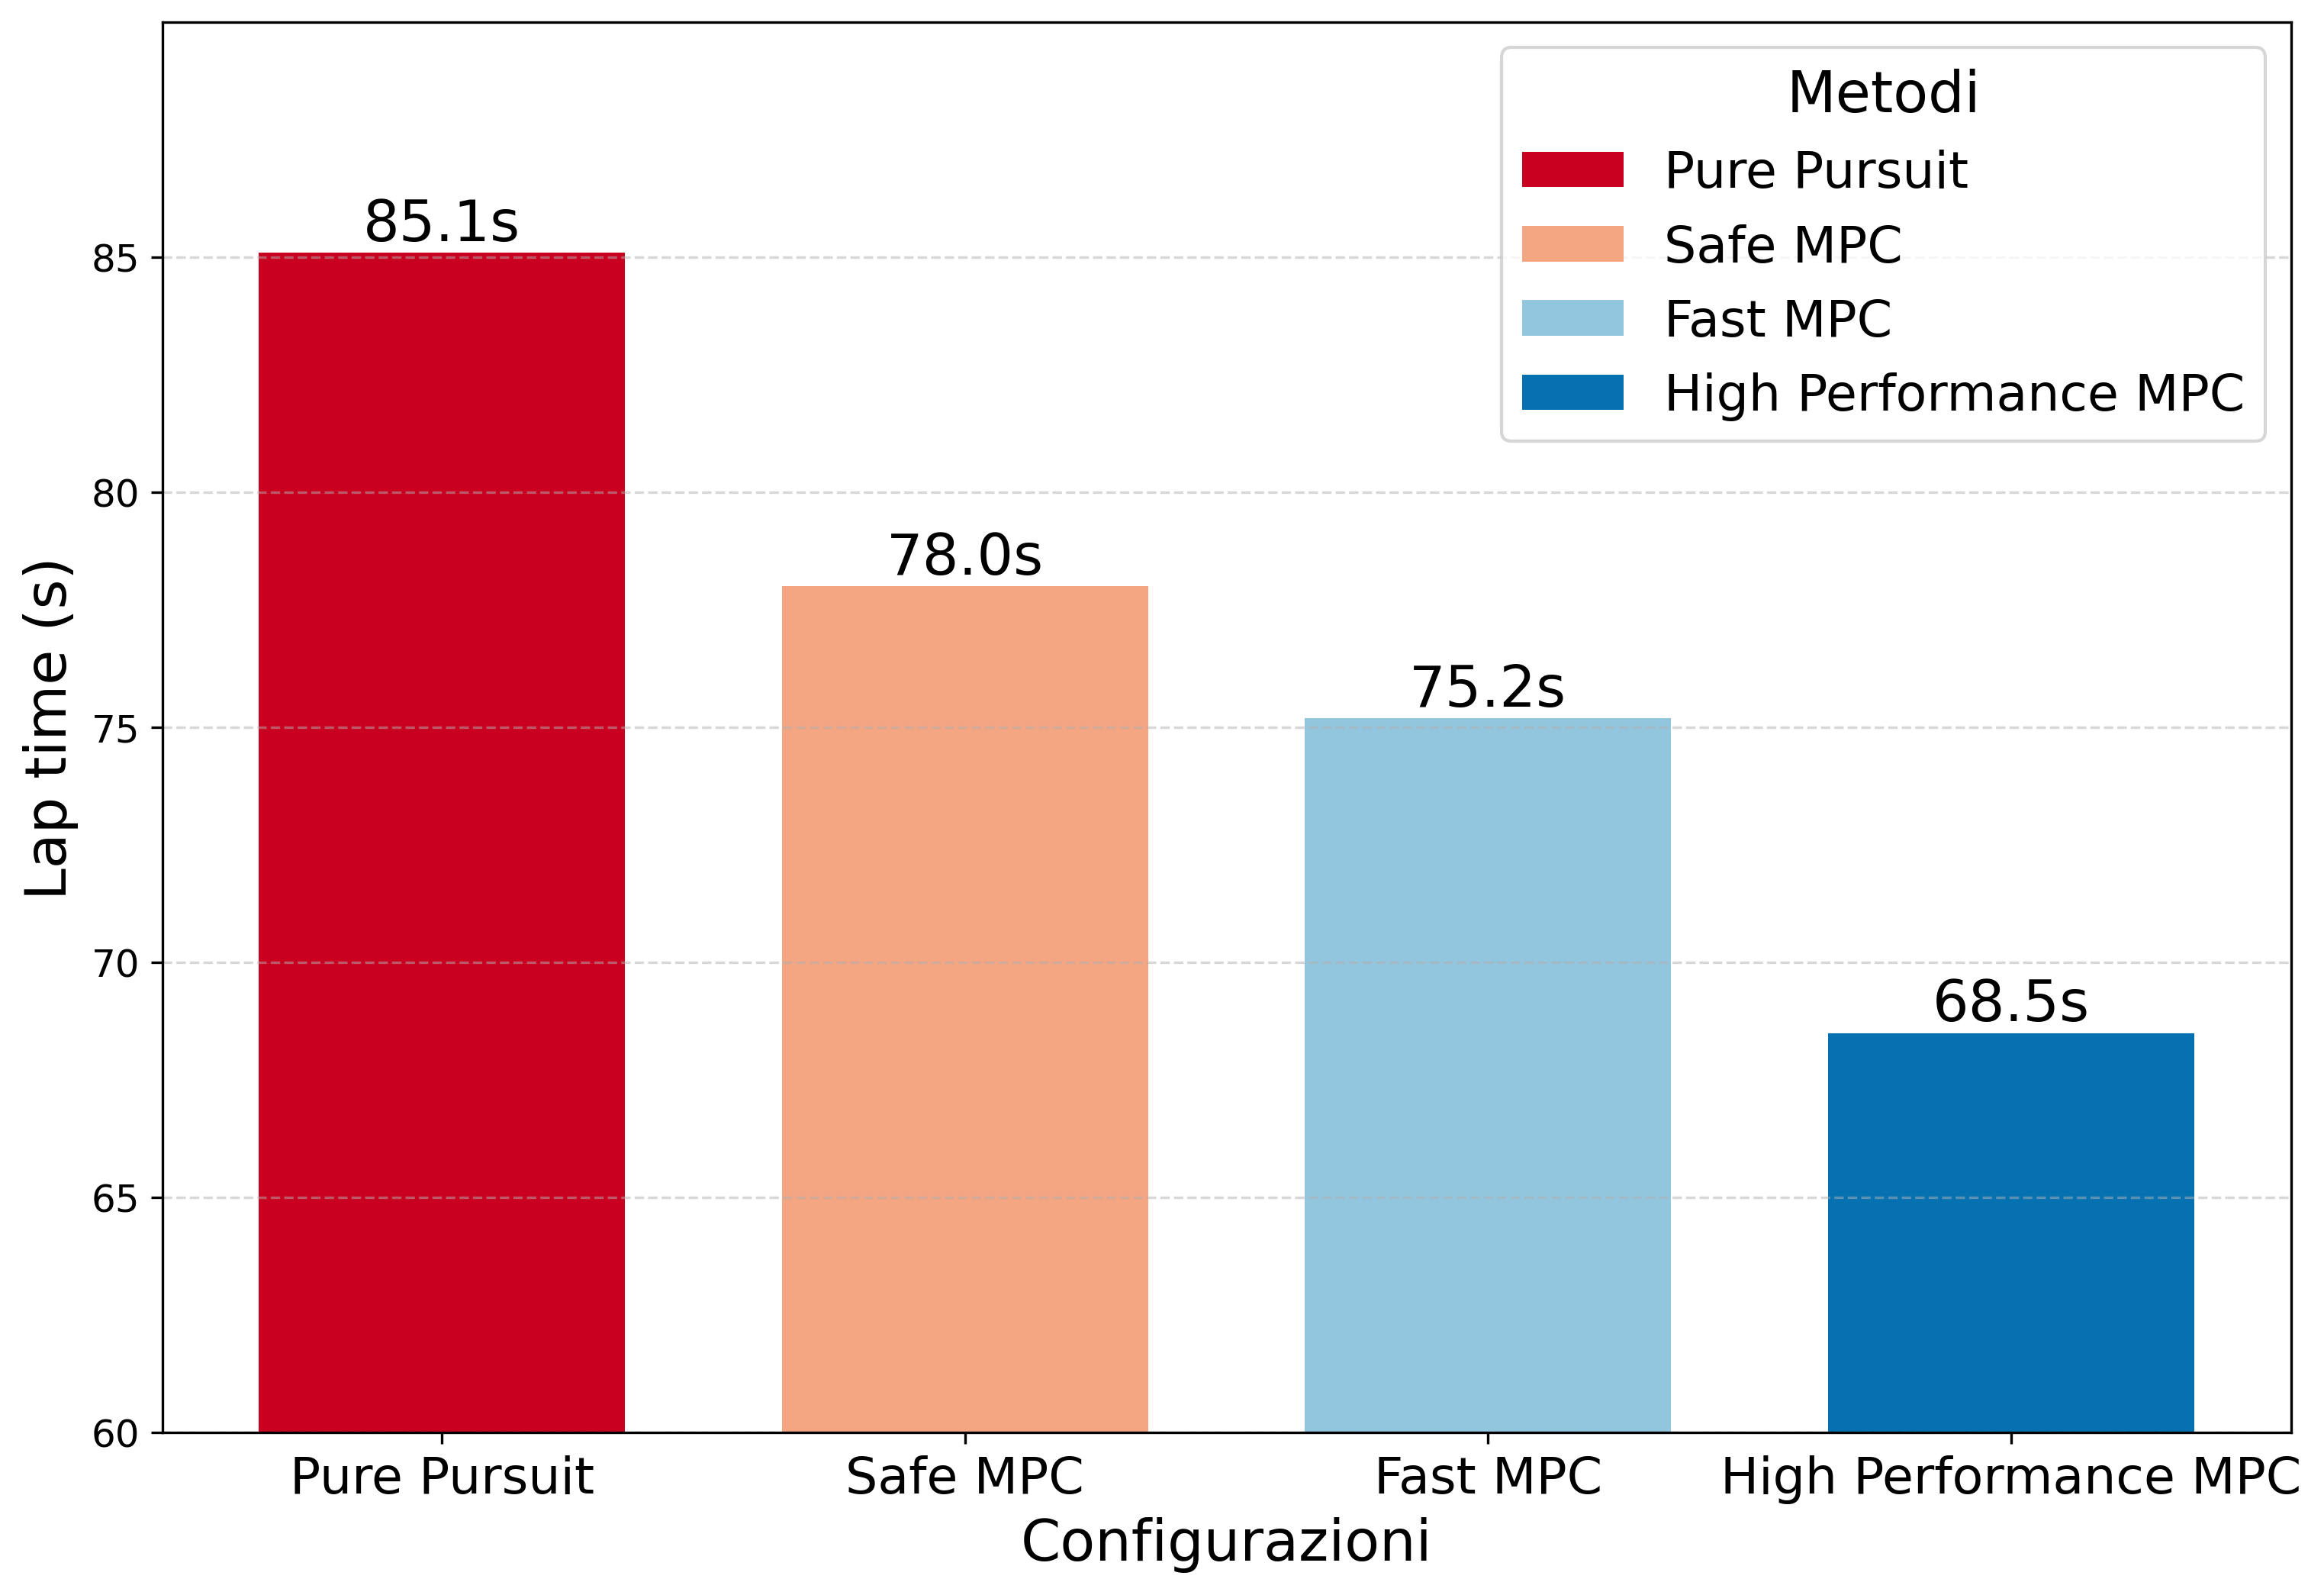
\includegraphics[width=\textwidth]{images/spa_lap_time_comparisons.png} 
        \caption{\textit{Spa}}
        \label{fig:laptime_spa}
    \end{subfigure}
    %\vfill
    \begin{subfigure}[b]{0.49\textwidth}
        \centering
        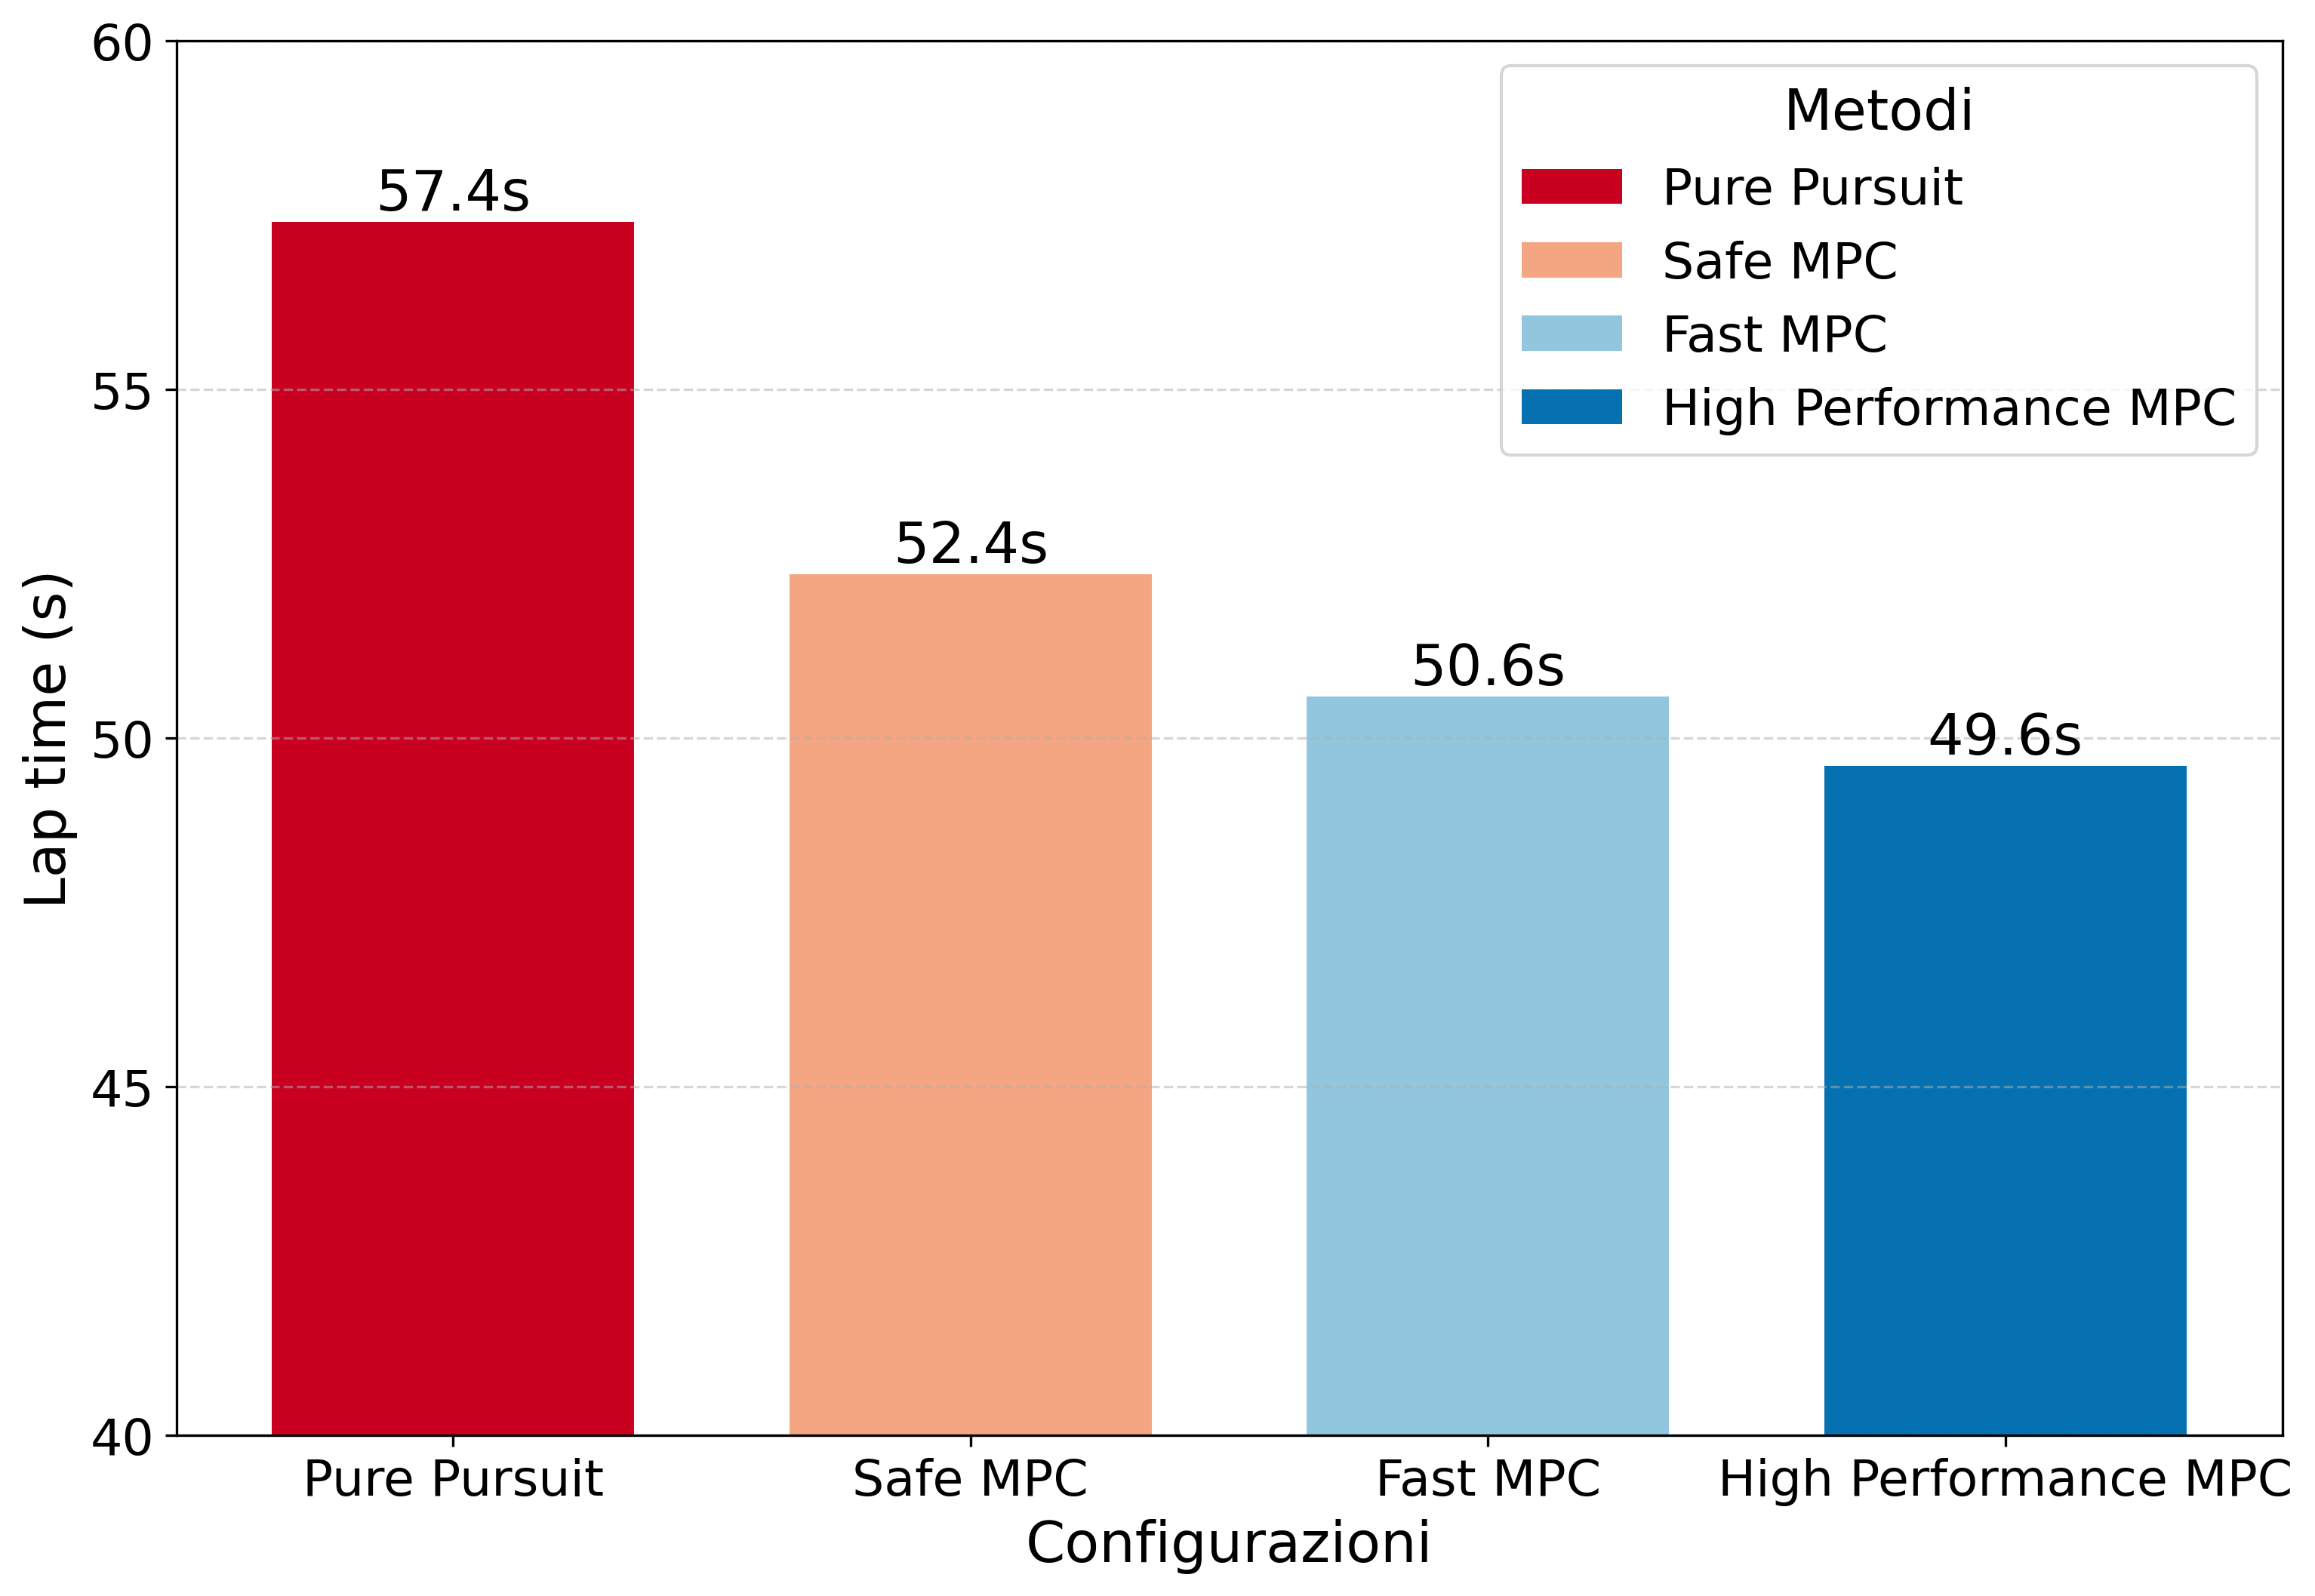
\includegraphics[width=\textwidth]{images/monza_lap_time_comparisons.png}
        \caption{\textit{Monza}}
        \label{fig:laptime_monza}
    \end{subfigure}
    \caption{Lap time per ogni metodo di controllo misurato.}
    \label{fig:fig13} % etichetta utilizzata per riferisi all'immagine
\end{figure}
Si possono osservare in Fig.~\ref{fig:fig13} i tempi per \textit{Pure Pursuit}
e per ciascuna configurazione di \textit{Model Predictive Control}.
Essi rispecchiano le aspettative: il metodo col \textit{lap time} inferiore risulta essere 
\textit{High Performance MPC}, seguito dai metodi \textit{Fast} e \textit{Safe}. 
Invece, \textit{Pure Pursuit} richiede più tempo per completare un giro e, provando a farlo 
correre ripetutamente, tende ad andare a sbattere con più frequenza per via della semplicità di 
questo metodo di controllo \textit{reattivo} e \textit{geometrico}.

\subsection{Traiettorie}
Per visualizzare le traiettorie, essendo molto ravvicinate tra loro, si utilizzano degli
\textit{zoom} su delle zone specifiche del tracciato, ovvero un \textit{rettilineo} e 
alcune tipologie di curve che sono molto comuni nelle piste di \textit{Formula 1}:
\begin{enumerate}
    \item \textit{Chicane} -- Si tratta di una curva seguita da un'altra 
    curva nella direzione opposta che viene introdotta in un tratto 
    rettilineo di una pista per rallentare la velocità dei veicoli. 
    Può essere utilizzata per testare quanta velocità il veicolo riesce a portare verso 
    l'\textit{apex} (centro curva) -- il punto più interno seguito in una curva -- in entrambe le 
    curve, e con quanto anticipo ciò consente al sistema di accelerare in uscita dalla curva.
    \item \textit{Tornante} -- È una svolta di 180 gradi che permette di verificare il modo in cui 
    il sistema raggiunge l'\textit{apex} e, soprattutto, come entra ed esce dalle curve.
\end{enumerate}
Il circuito di \textit{Spa} presenta delle curve \textit{chicane} e un 
\textit{tornante}. Come visibile dalla Fig.~\ref{fig:fig14}, le traiettorie 
relative ai profili di \textit{MPC} sono più uniformi, poiché l'algoritmo ottimizza
sempre \textit{``online''}, e tendono a tagliare prima nelle curve rispetto al riferimento della 
\textit{raceline}. Le differenze tra i profili di \textit{MPC} sono dovute prettamente ai diversi
valori dell'orizzonte temporale e delle matrici di pesi, concetti già discussi nel 
Capitolo~\ref{chap:chap3}, da un punto di vista teorico, e nel Capitolo~\ref{chap:chap4} a livello implementativo.

A differenza di \textit{MPC}, \textit{Pure Pursuit} ha un andamento 
più variabile, poiché tende a correggere l'angolo di sterzata con elevata frequenza, per seguire
il più possibile i waypoints della \textit{raceline} a cui fa riferimento. 
Quanto descritto lo si può notare specialmente nella curva a gomito della 
Fig.~\ref{fig:curva_spa}, nella quale \textit{HP MPC} taglia molto in anticipo rispetto a tutti gli altri.

\begin{figure}[H]
    \centering
    \begin{subfigure}[b]{0.49\textwidth}
        \centering
        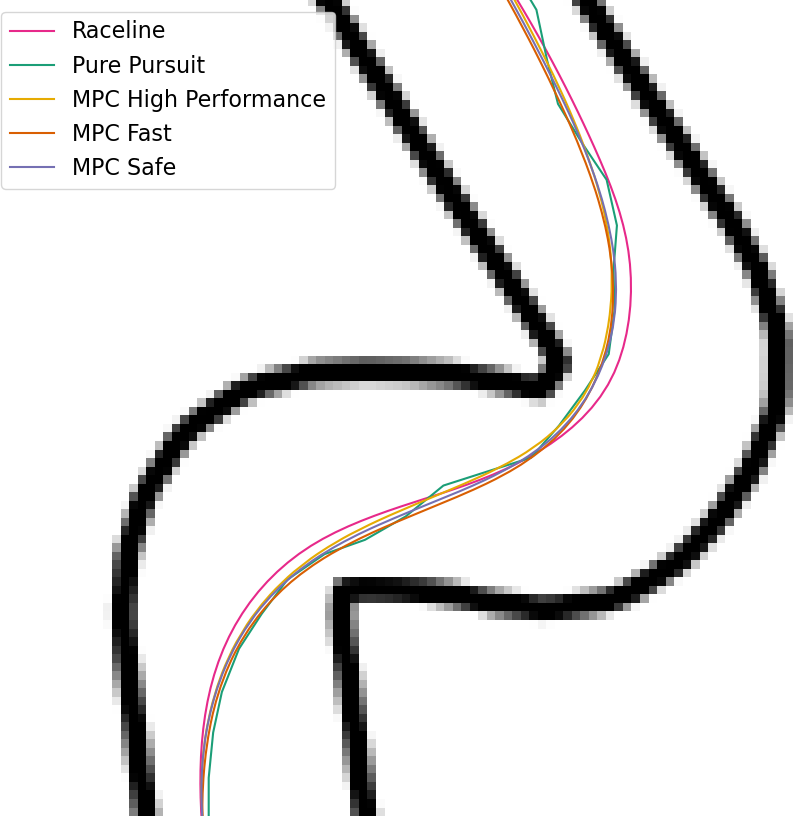
\includegraphics[width=\textwidth]{images/spa_traj_comparison_chicane.png} 
        \caption{Chicane}
        \label{fig:chic_spa}
    \end{subfigure}
    \hfill
    \begin{subfigure}{0.49\textwidth}
        \centering
        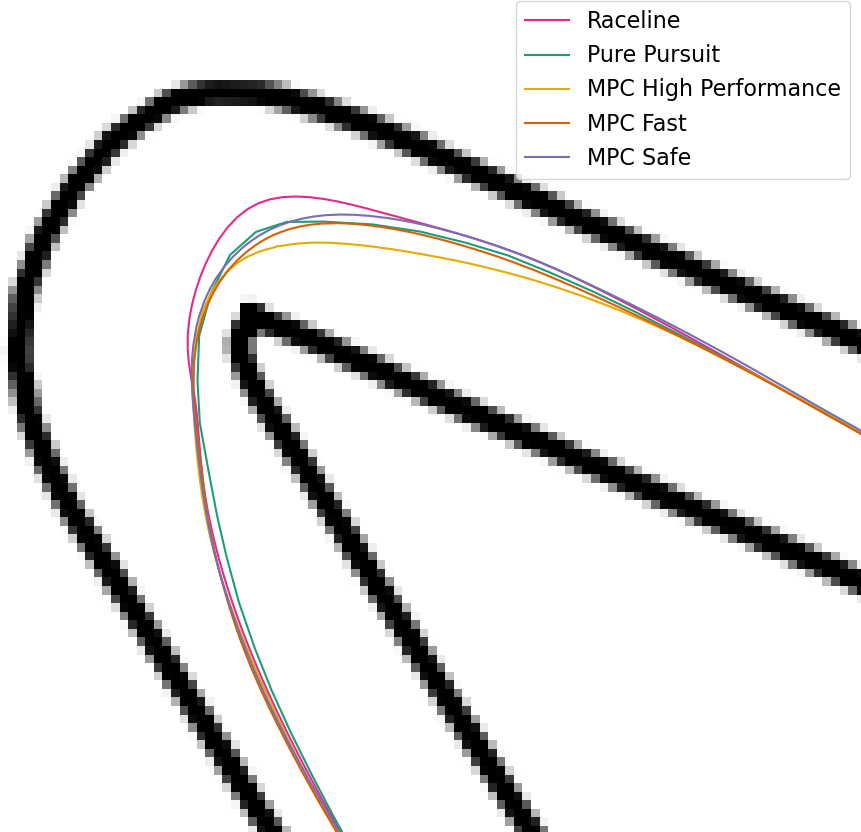
\includegraphics[width=\textwidth]{images/spa_traj_comparison_curva.png}
        \caption{Curva a gomito}
        \label{fig:curva_spa}
    \end{subfigure}
    \begin{subfigure}[b]{0.50\textwidth}
        \centering
        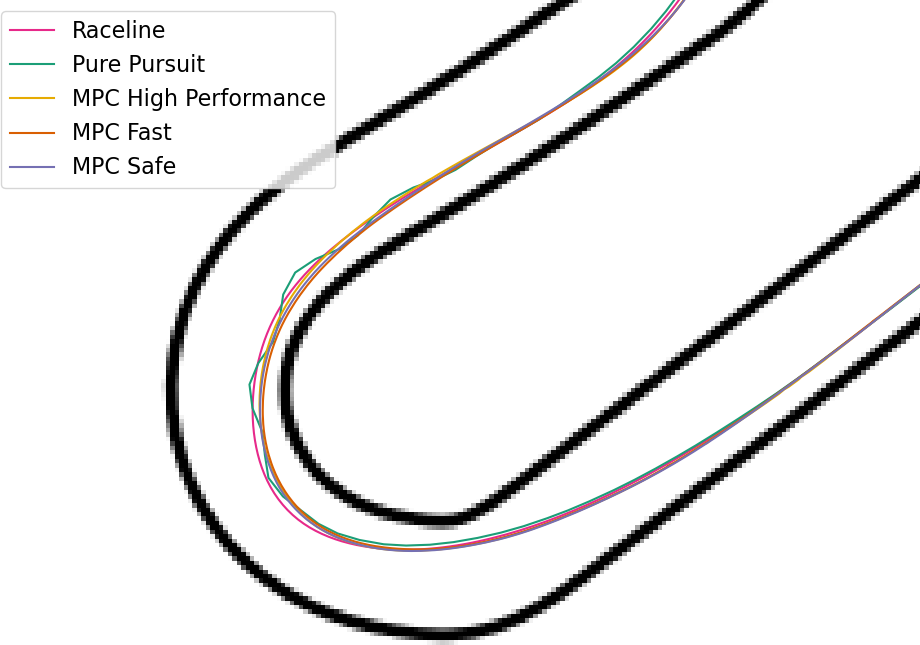
\includegraphics[width=\textwidth]{images/spa_traj_comparison_tornante.png}
        \caption{Tornante}
        \label{fig:torn_spa}
    \end{subfigure}
    \caption{Diversi tipi di curve su \textit{Spa}.}
    \label{fig:fig14} % etichetta utilizzata per riferisi all'immagine
\end{figure}

Si può notare in Fig.~\ref{fig:fig15} un comportamento simile anche per il circuito di Monza, 
composto prettamente da chicane e da rettilinei. Questi ultimi sono visualizzati per entrambe
le piste nella Fig.~\ref{fig:fig16}, in modo da evidenziare la vicinanza di tutte le traiettorie, 
che risultano di fatto sovrapposte.

\begin{figure}[H]
    \centering
    \begin{subfigure}[b]{0.49\textwidth}
        \centering
        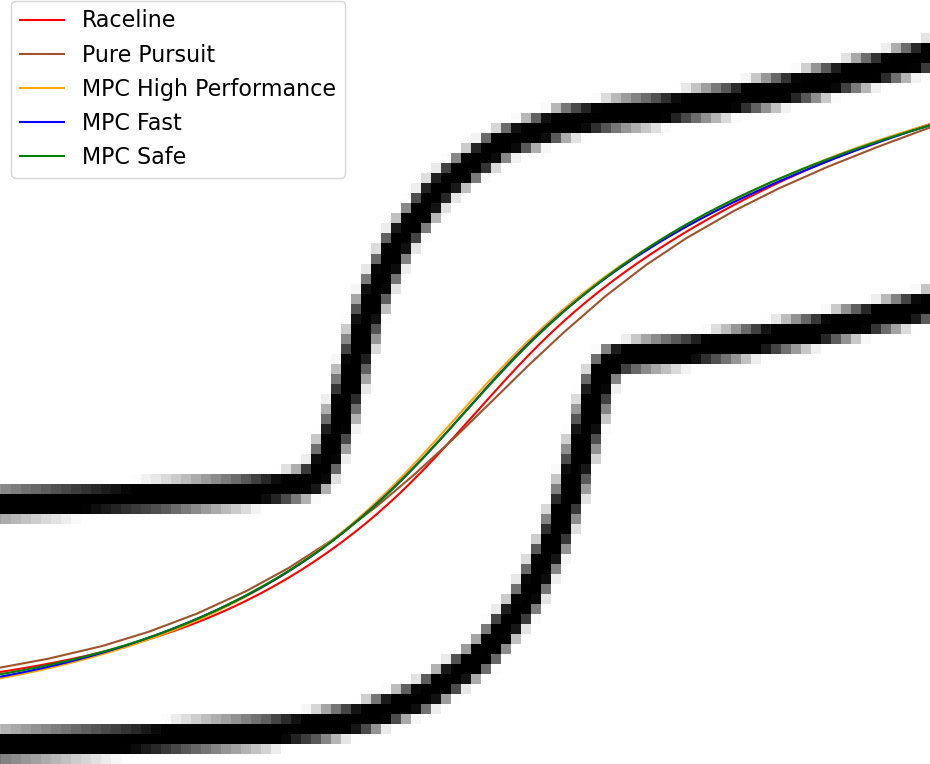
\includegraphics[width=\textwidth]{images/monza_traj_comparison_chicane.png} 
        \caption{Prima Chicane}
        \label{fig:chic_monza}
    \end{subfigure}
    \hfill
    \begin{subfigure}[b]{0.49\textwidth}
        \centering
        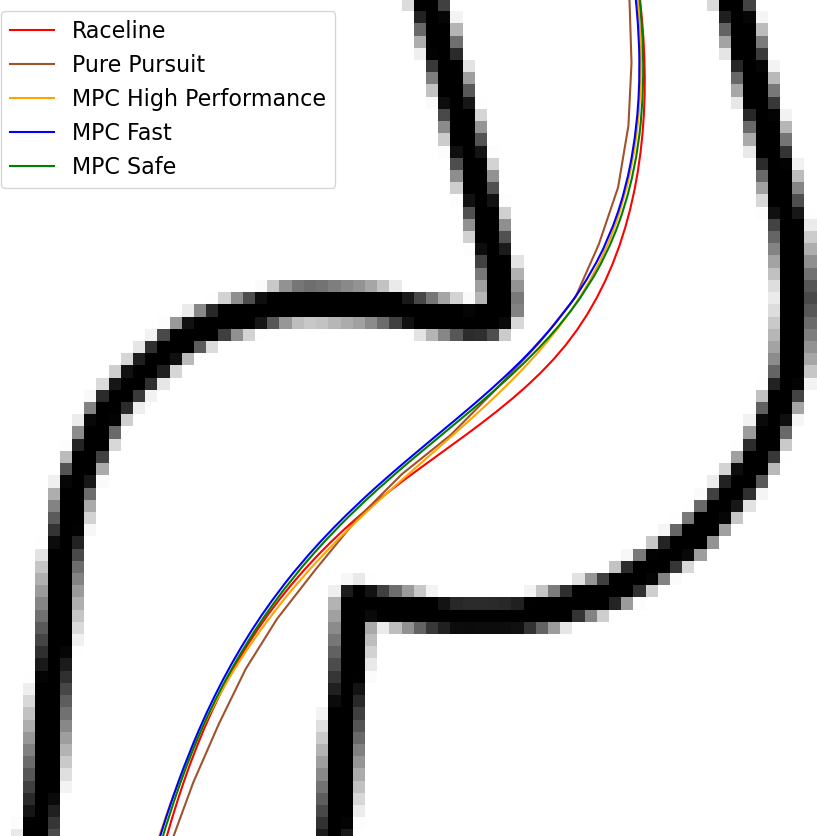
\includegraphics[width=\textwidth]{images/monza_traj_comparison_chicane2.png}
        \caption{Seconda Chicane}
        \label{fig:chic2_monza}
    \end{subfigure}
    \caption{Curve su \textit{Monza}.}
    \label{fig:fig15} % etichetta utilizzata per riferisi all'immagine
\end{figure}
\begin{figure}[H]
    \centering
    \begin{subfigure}[b]{0.49\textwidth}
        \centering
        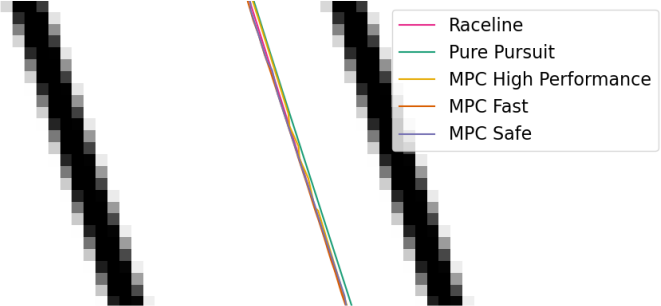
\includegraphics[width=\textwidth]{images/spa_trajectory_comparison_straight.png} 
        \caption{\textit{Spa}}
        \label{fig:str_spa}
    \end{subfigure}
    \hfill
    \begin{subfigure}[b]{0.49\textwidth}
        \centering
        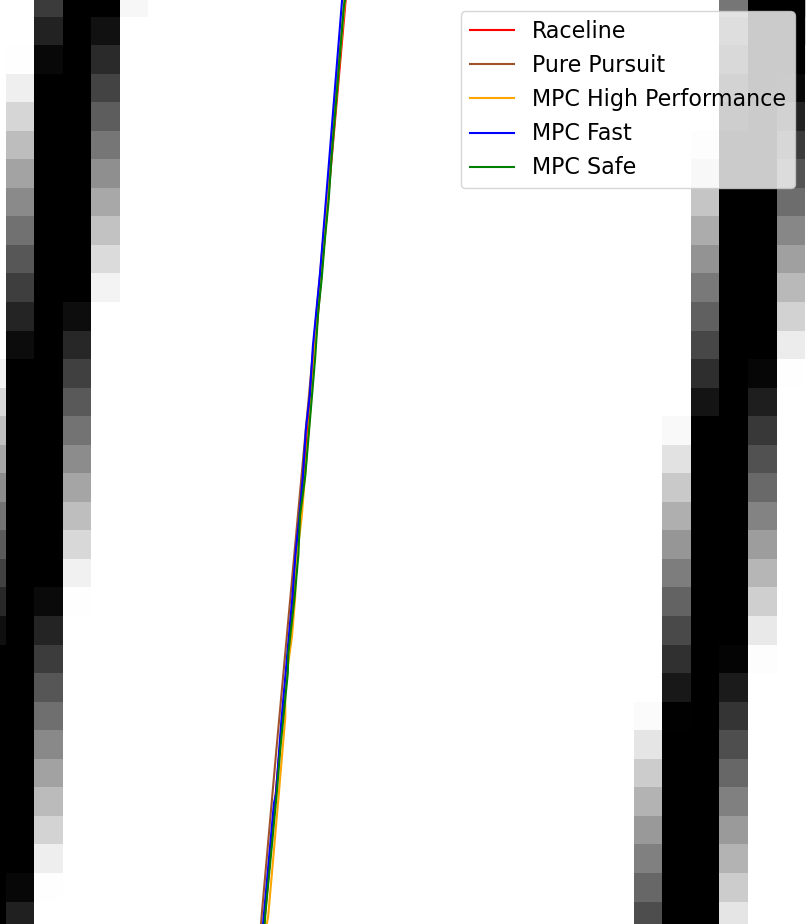
\includegraphics[width=0.8\textwidth]{images/monza_trajectory_comparison_straight.png}
        \caption{\textit{Monza}}
        \label{fig:str_monza}
    \end{subfigure}
    \caption{Rettilinei su \textit{Monza} e \textit{Spa}.}
    \label{fig:fig16} % etichetta utilizzata per riferisi all'immagine
\end{figure}

%    %\centering
%    %\includegraphics[scale=0.4]{images/%monza_mpc_safe_crosstrack_error.png}\hspace{0.02cm}
%    \includegraphics[scale=0.4]{images/monza_mpc_fast_crosstrack_error.png}


\subsection{Crosstrack Error}
Nella sezione~\ref{subs:metrics}, relativa alle metriche, è stato introdotto il 
\textit{Crosstrack Error}, detto anche errore di tracking. Tuttavia, questo dato è stato usato
esclusivamente per mostrare la \textit{deviazione massima} e, soprattutto, per calcolare l'\textit{RMSE}, in 
modo da avere una misura accurata che indica di quanto si discosta in media l'errore di tracking 
dallo zero, cioè il caso con valore teorico e valore corrente identici. 
Si vuole però dare anche un'idea visiva dell'evoluzione dell'errore di tracking, sempre attraverso la realizzazione di un grafico. 
Nella Fig.~\ref{fig:fig17} viene mostrato, per entrambe le piste, l'errore di tracking generato 
dal \textit{Pure Pursuit} che, come confermato dall'RMSE, ha valori mediamente superiori. 
Pertanto, questo metodo è stato utilizzato come \textit{baseline} anche per la scala cromatica in 
ogni grafico inerente a questa metrica. Si segnala che il triangolo indica la posizione di partenza del giro.

\begin{figure}[H]
    \centering
    \begin{subfigure}[b]{0.49\textwidth}
        \centering
        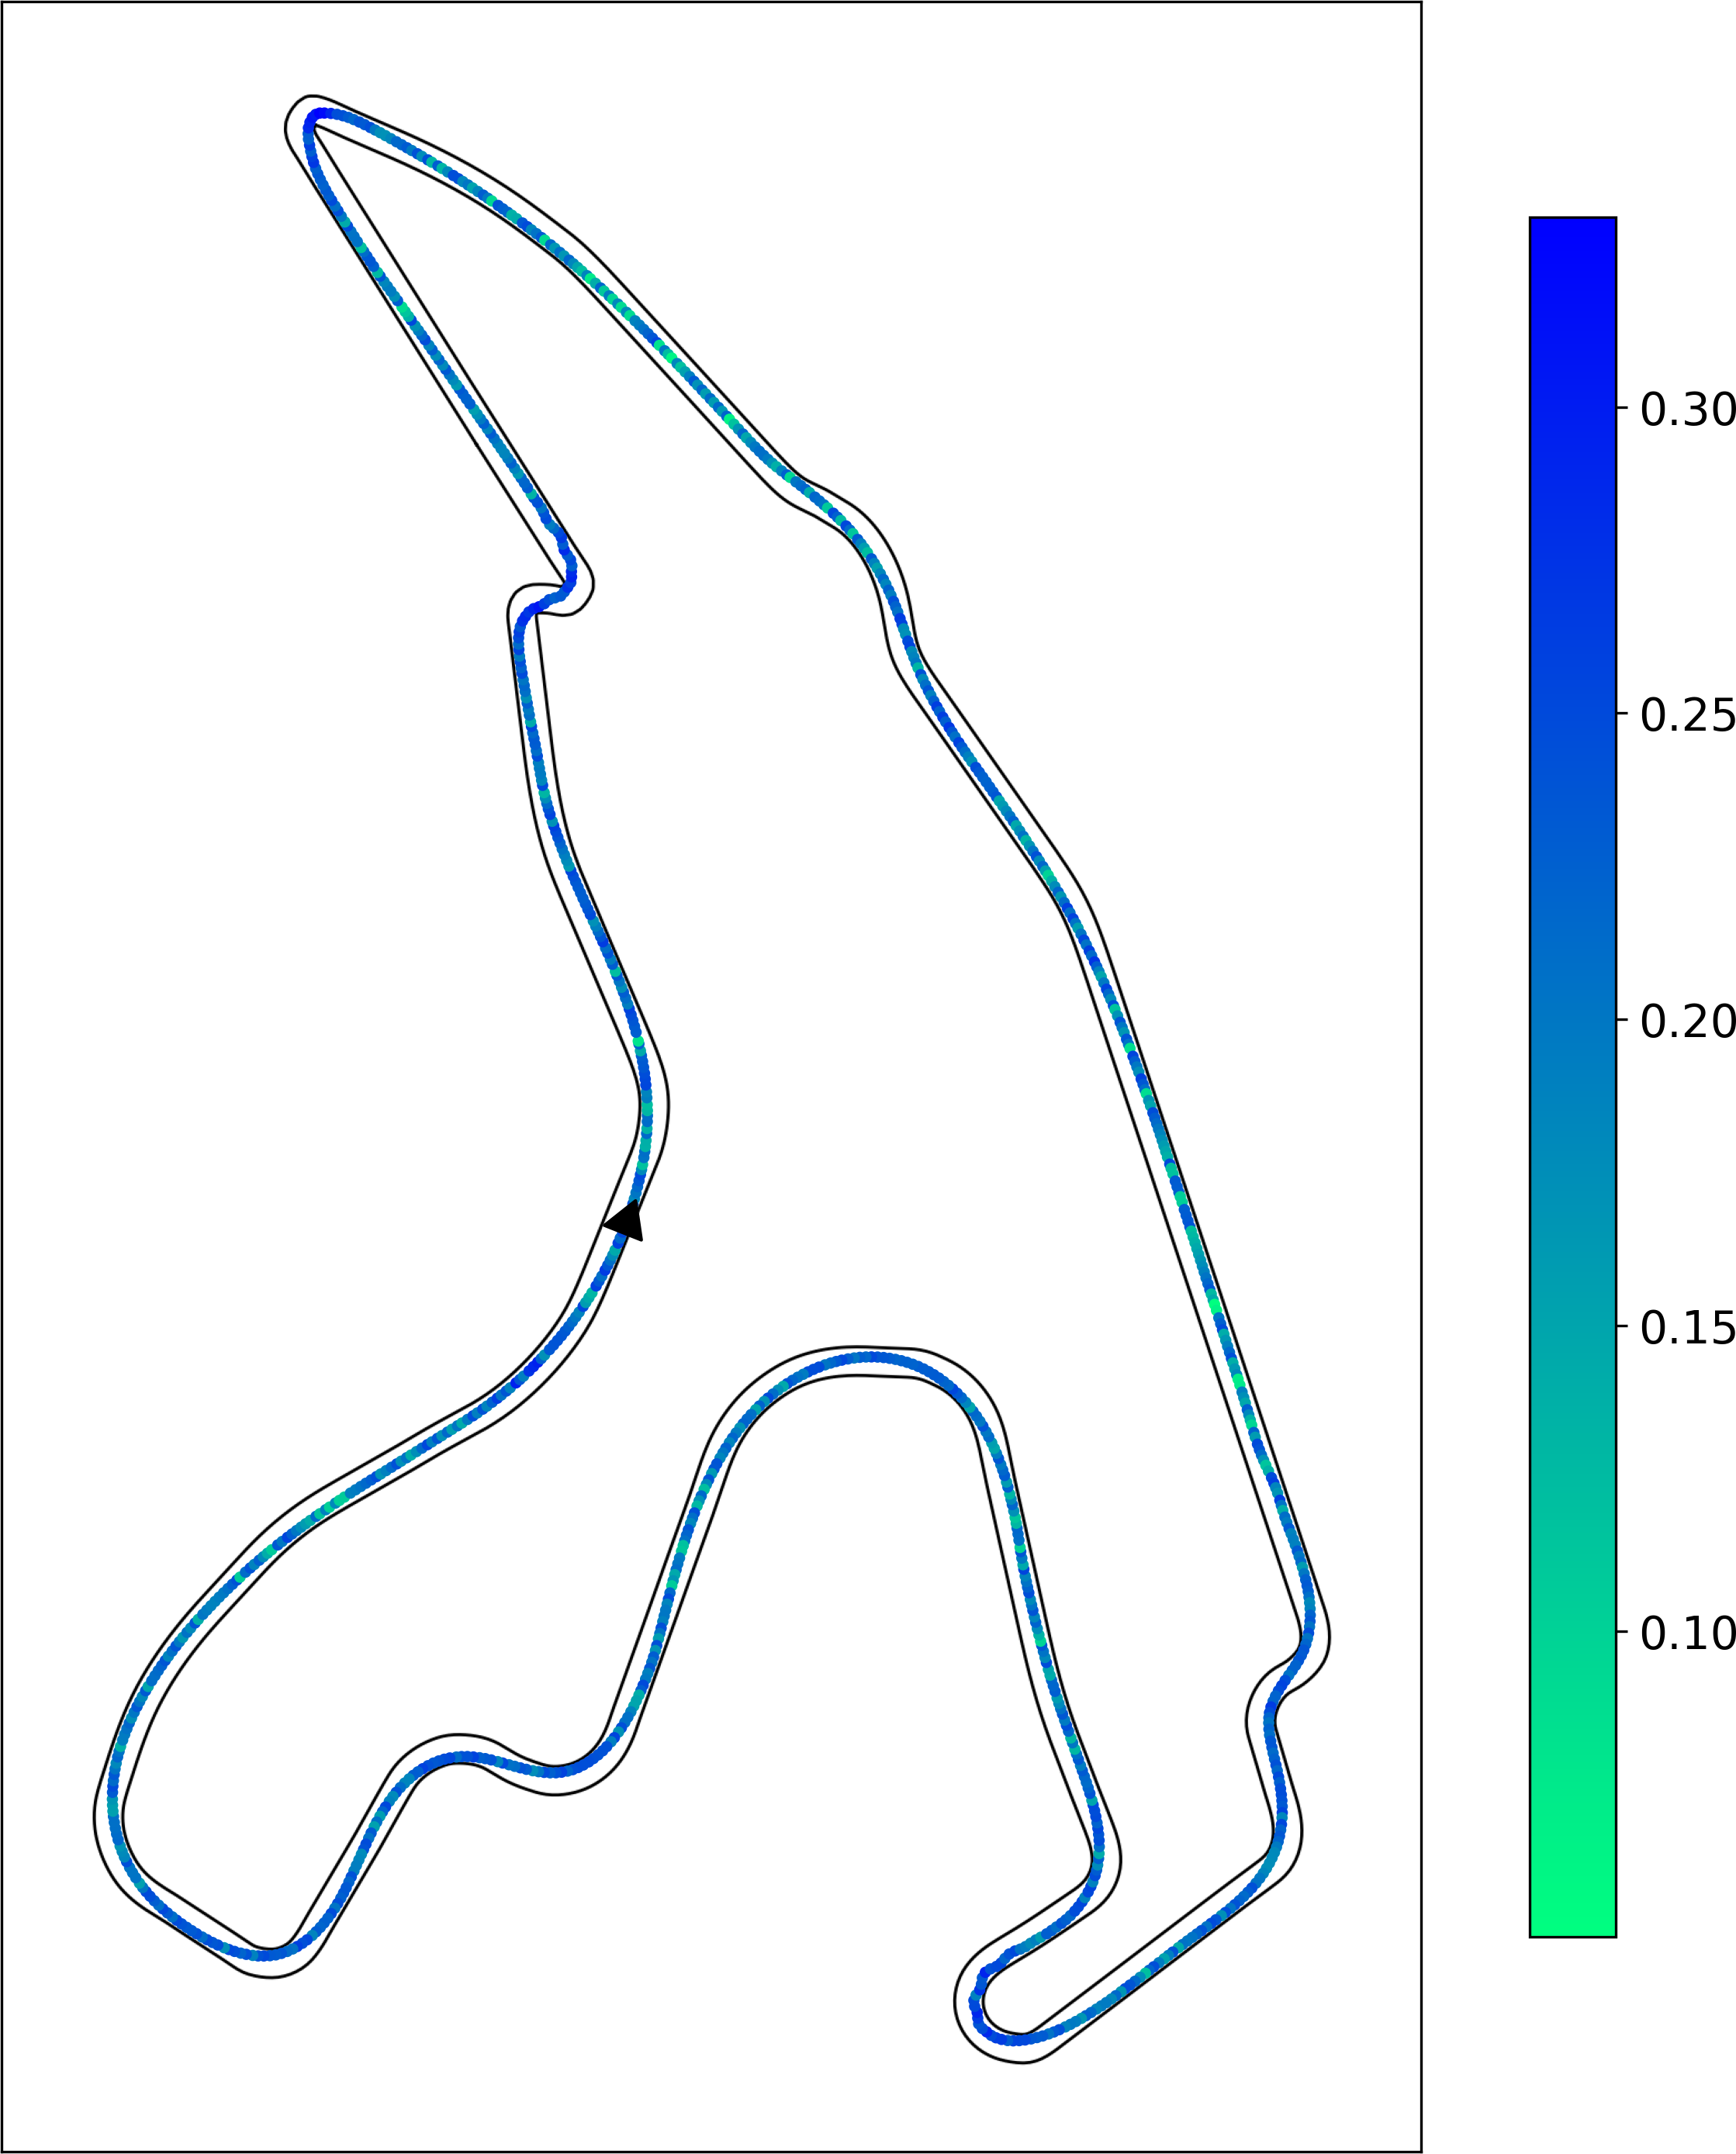
\includegraphics[width=0.75\textwidth]{images/spa_pp_crosstrack.png} 
        \caption{\textit{Spa}}
        \label{fig:tracking_pp_spa}
    \end{subfigure}
    %\hfill
    \begin{subfigure}[b]{0.469\textwidth}
        \centering
        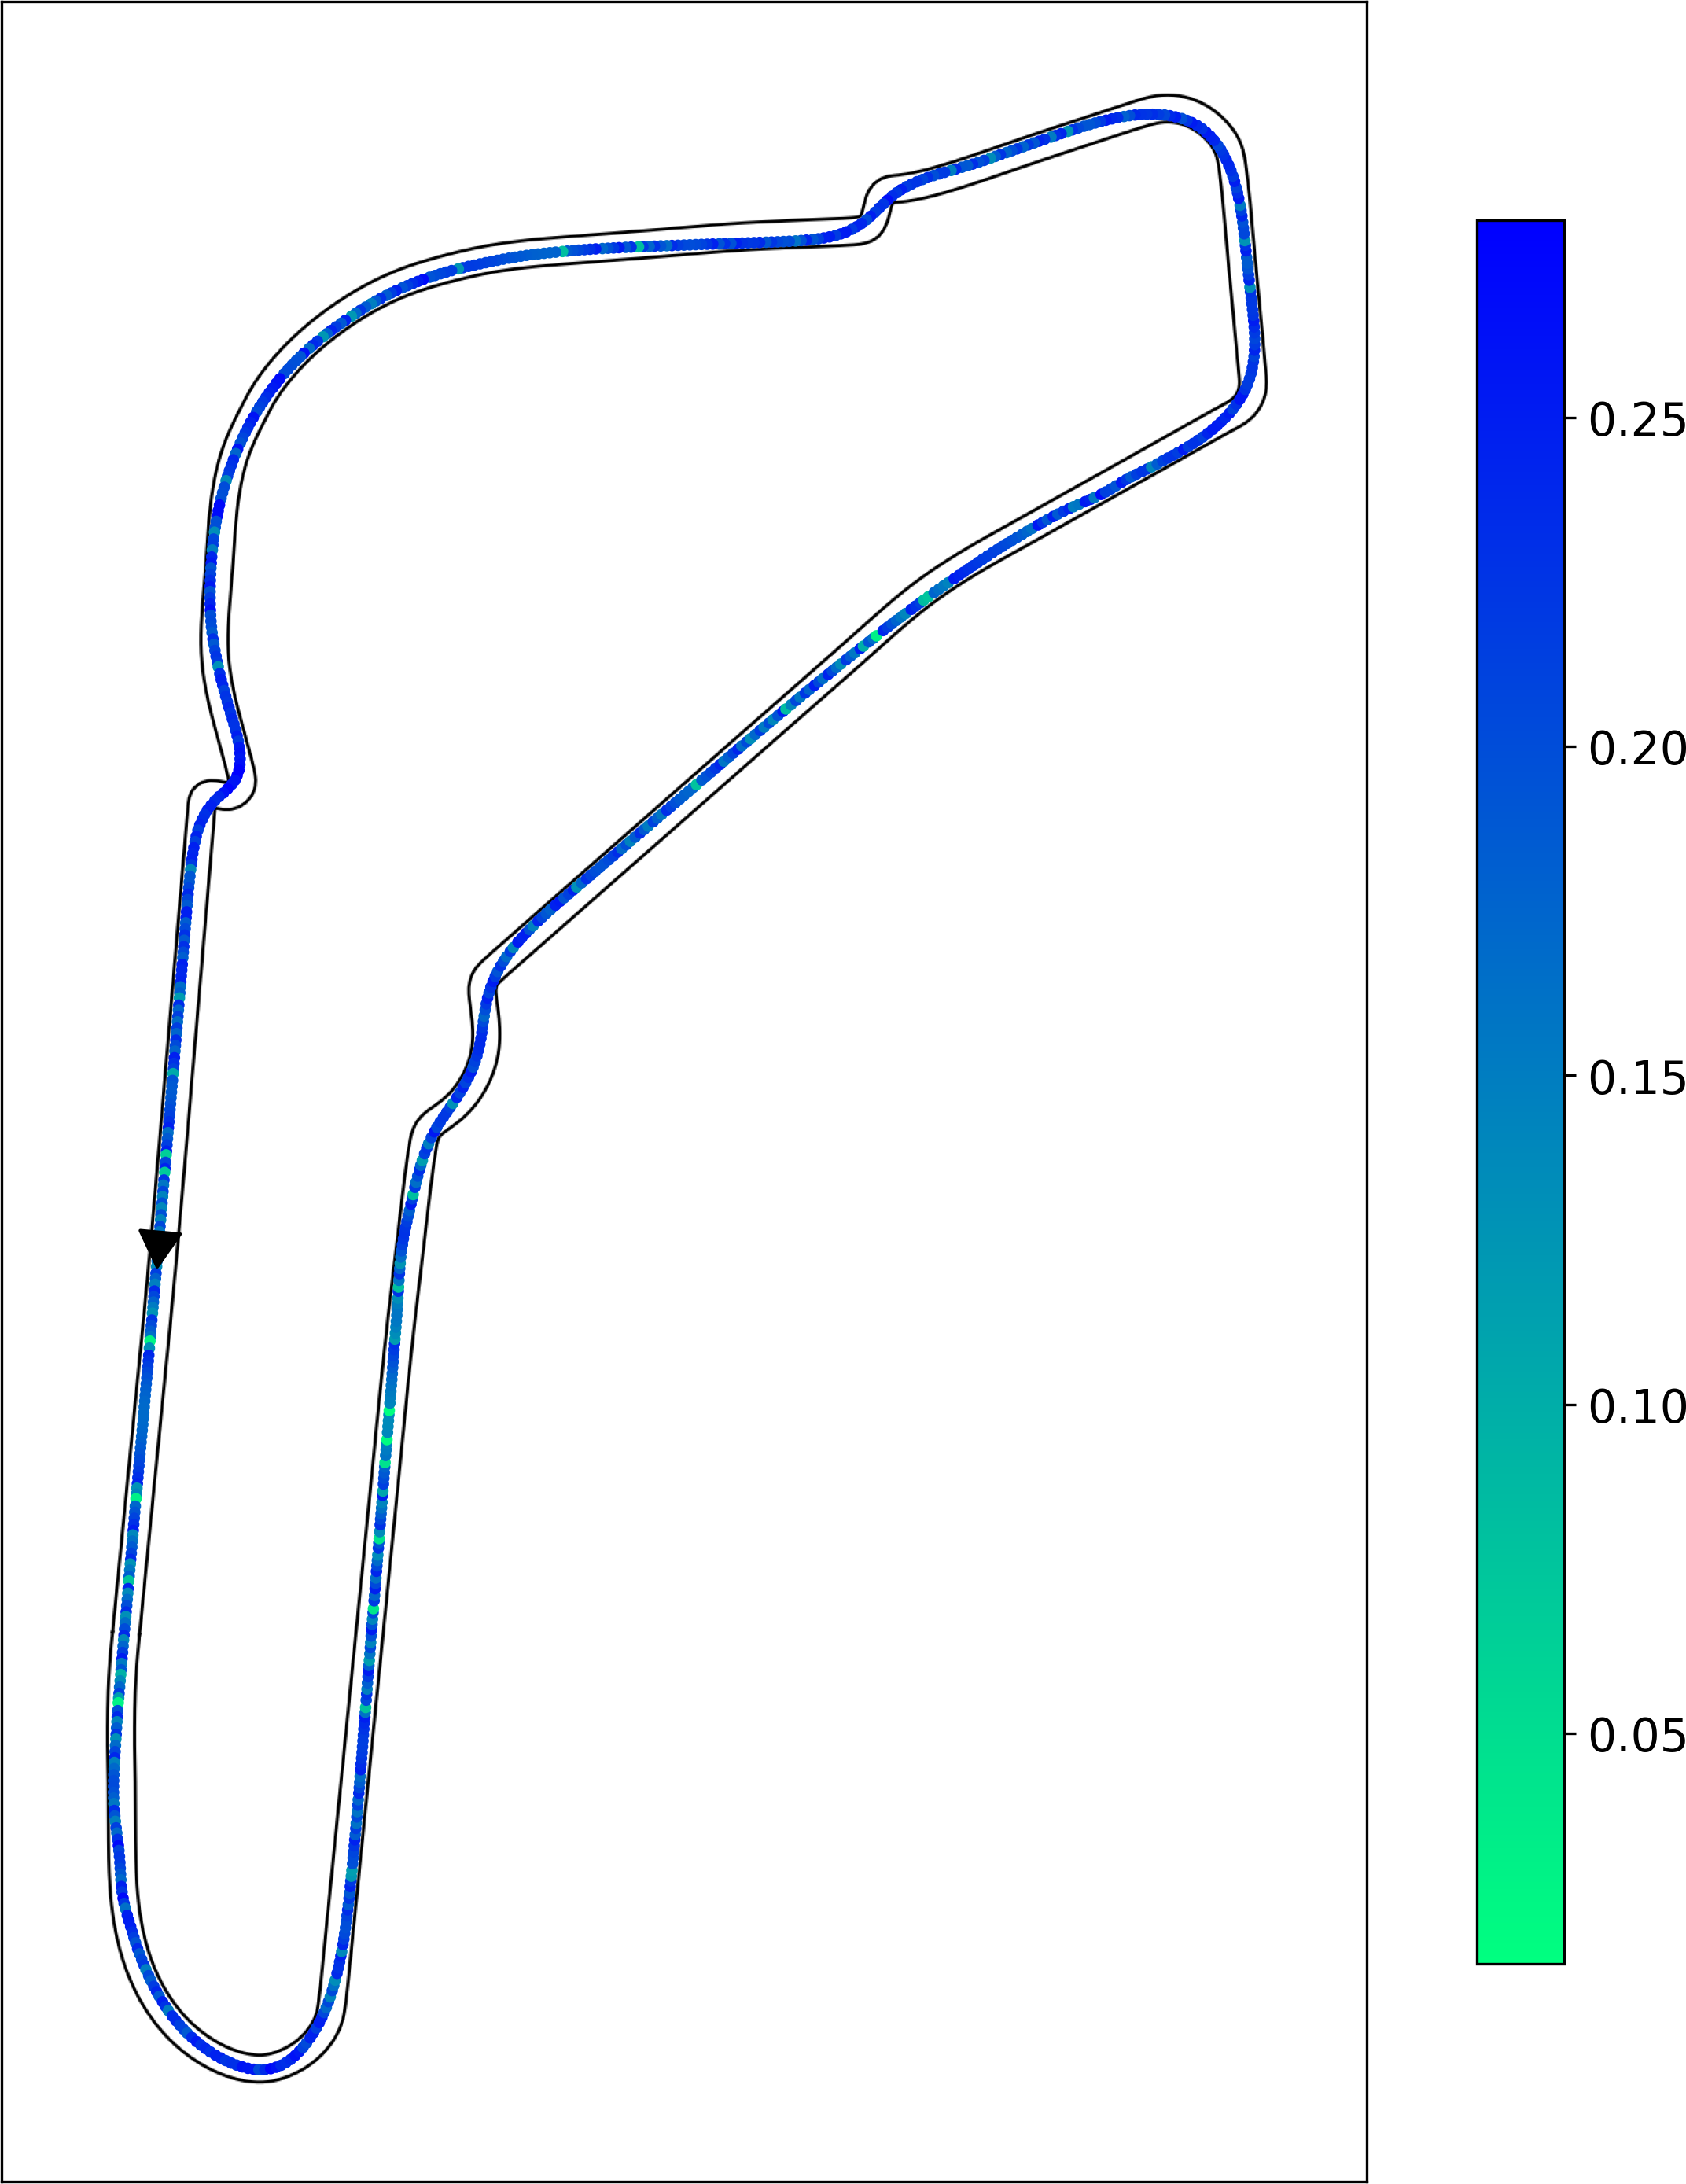
\includegraphics[width=0.75\textwidth]{images/monza_pp_crosstrack.png}
        \caption{\textit{Monza}}
        \label{fig:tracking_pp_monza}
    \end{subfigure}
    \caption{Crosstrack Error per \textit{Pure Pursuit}, usato come baseline.}
    \label{fig:fig17} % etichetta utilizzata per riferisi all'immagine
\end{figure}
Infatti, nella Fig.~\ref{fig:fig18} si noti
come tutti i profili di \textit{MPC} abbiano un colore più chiaro per 
la quasi totalità del percorso; in particolare, il profilo 
\textit{High Performance} è quello coi valori inferiori, seguito da 
\textit{Safe} -- confermando di riflesso il valore basso registrato per 
l'\textit{RMSE} -- e da \textit{Fast}. Inoltre, soprattutto per \textit{High Performance}, 
si può notare dal grafico il colore più marcato nella parte della 
\textit{curva a gomito} -- già vista nella Fig.~\ref{fig:curva_spa} -- 
poiché la ``taglia'' prima di ogni altro profilo.

\begin{figure}[H]
    \centering
    \begin{subfigure}[b]{0.3\textwidth}
        \centering
        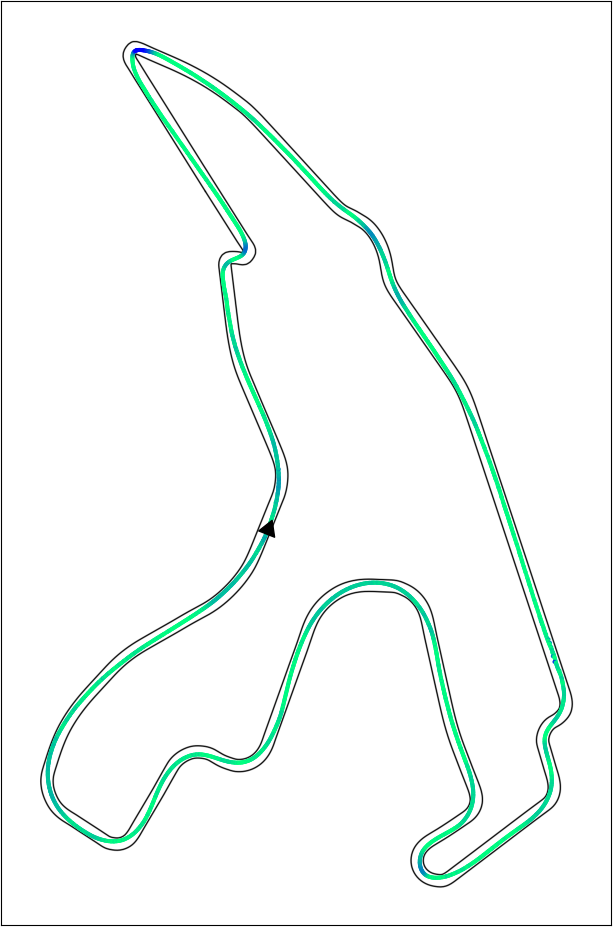
\includegraphics[width=\textwidth]{images/spa_mpc_hp_crosstrack.png} 
        \caption{\textit{High Performance}}
        \label{fig:tracking_hp_spa}
    \end{subfigure}
    %\hfill
    \begin{subfigure}[b]{0.3\textwidth}
        \centering
        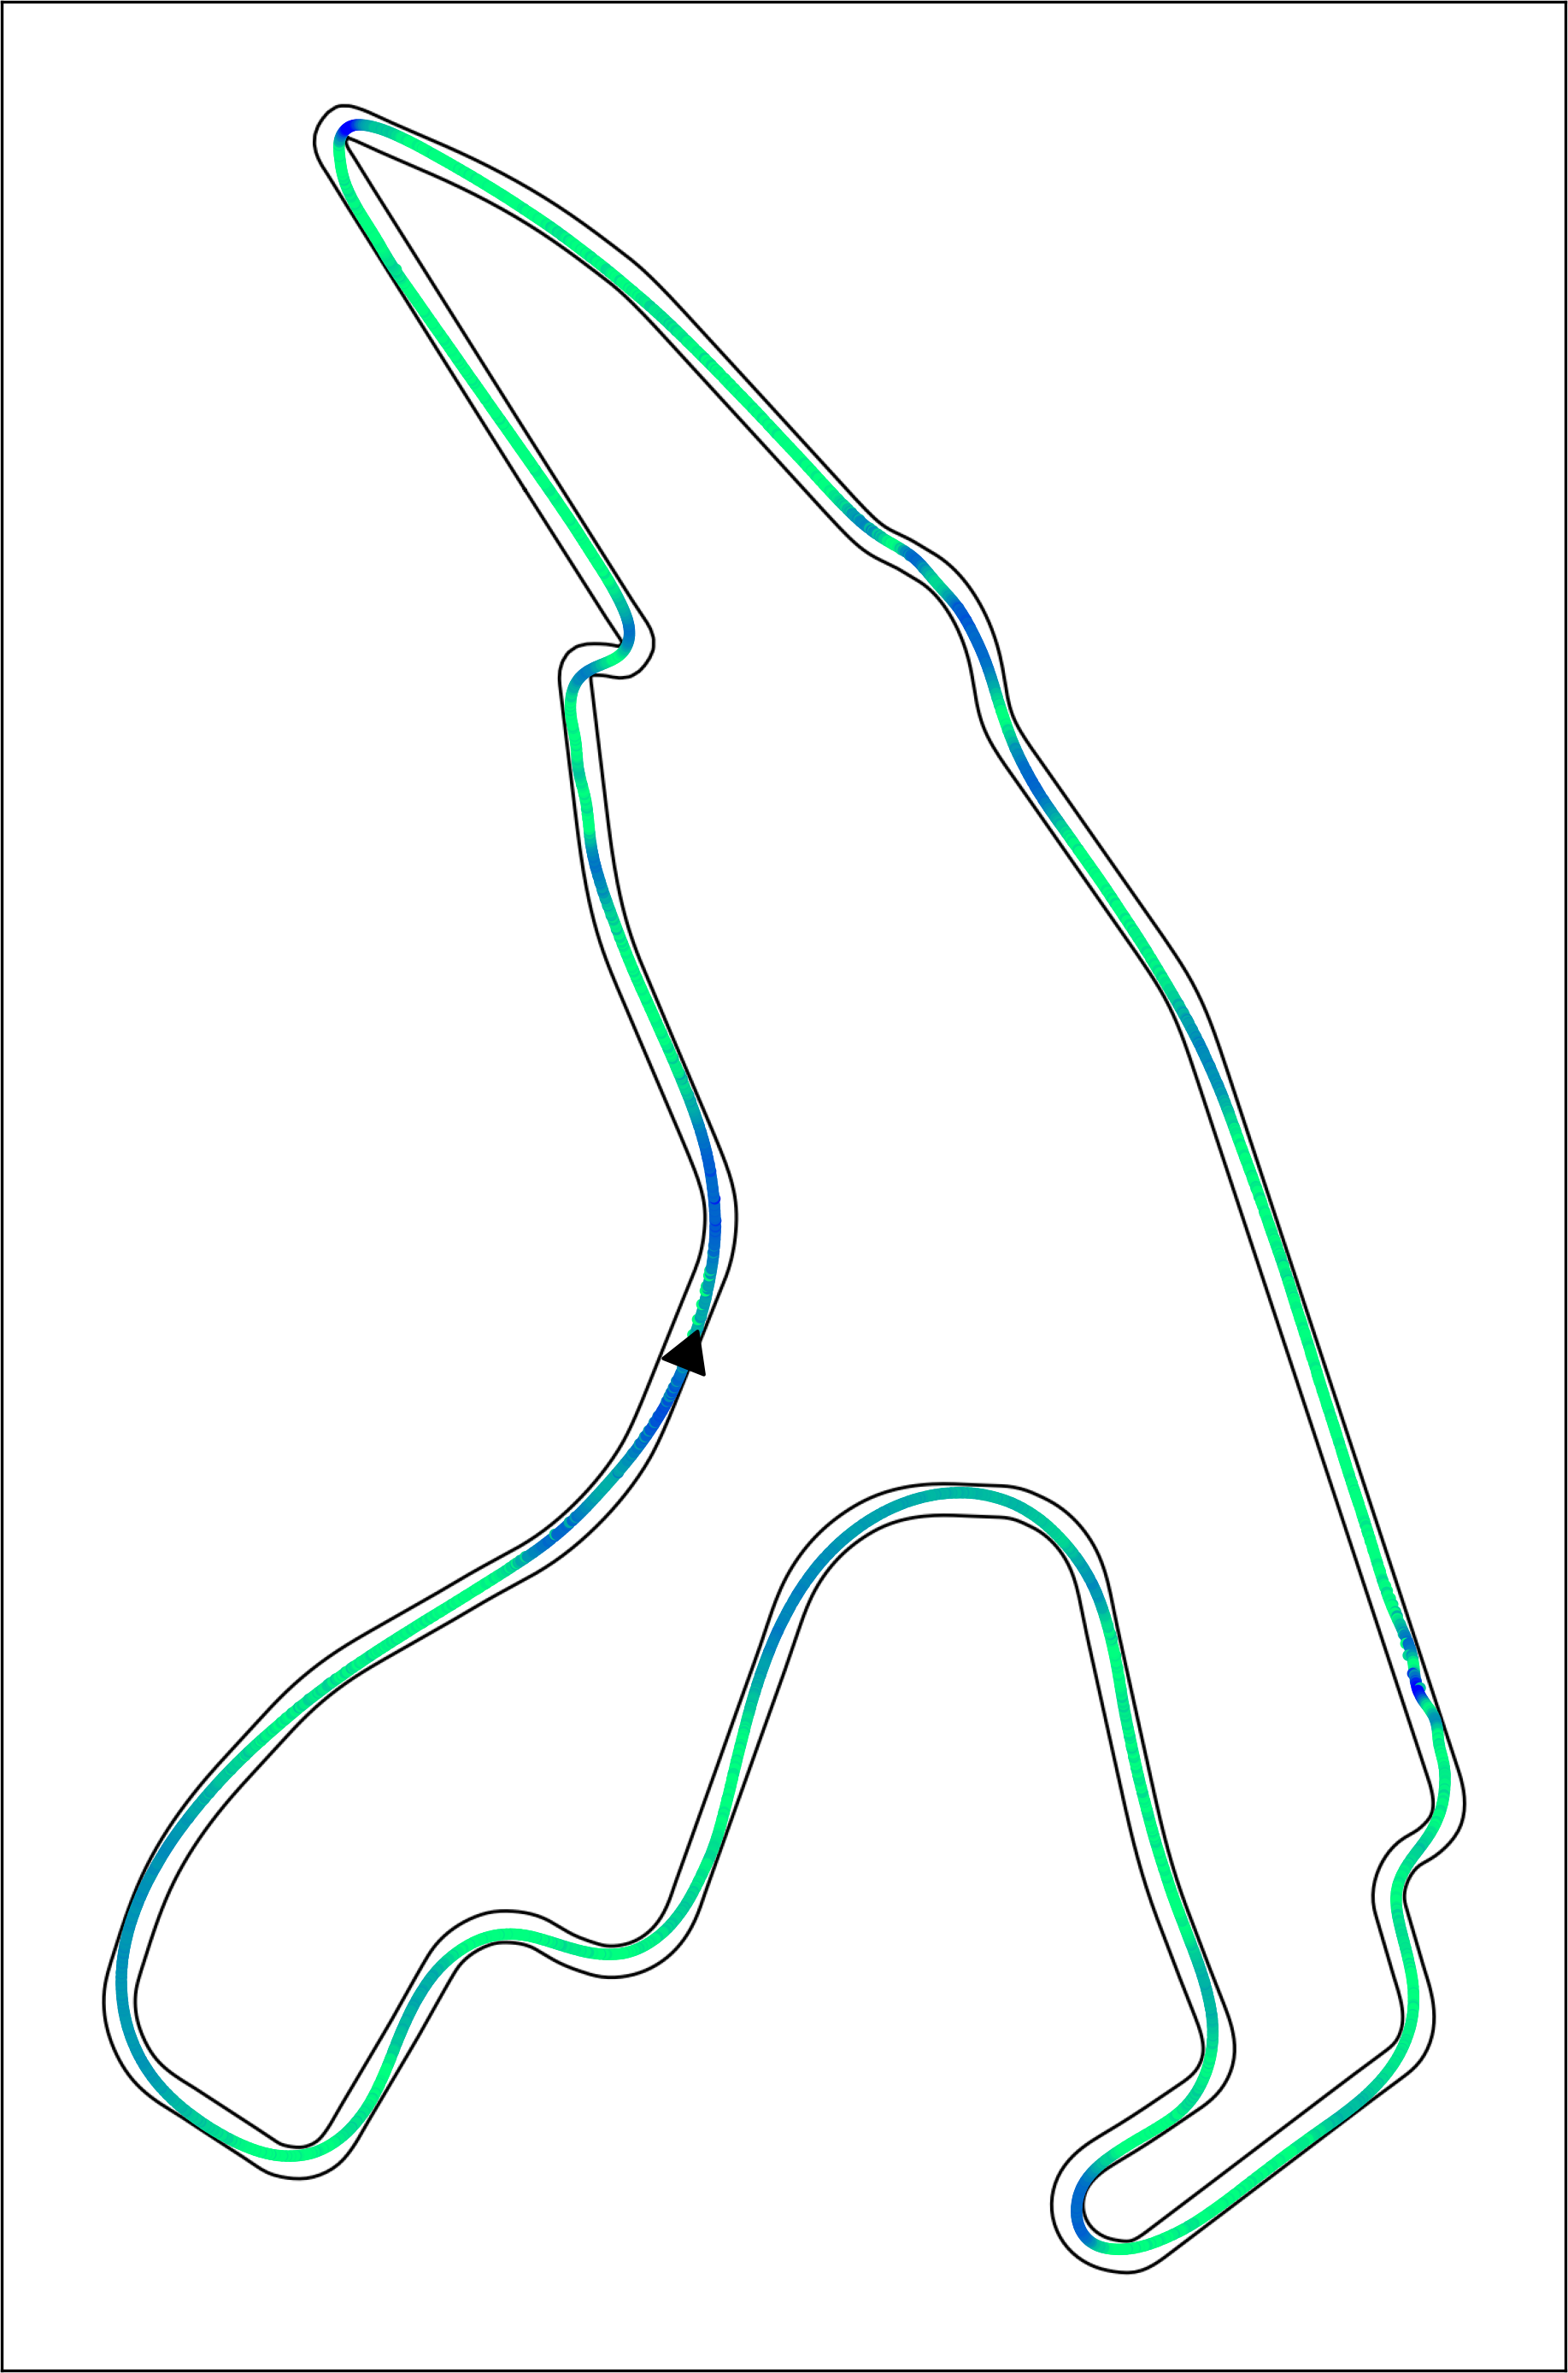
\includegraphics[width=\textwidth]{images/spa_mpc_fast_crosstrack.png}
        \caption{\textit{Fast}}
        \label{fig:tracking_fast_spa}
    \end{subfigure}
    %\hfill
    \begin{subfigure}[b]{0.366\textwidth}
        \centering
        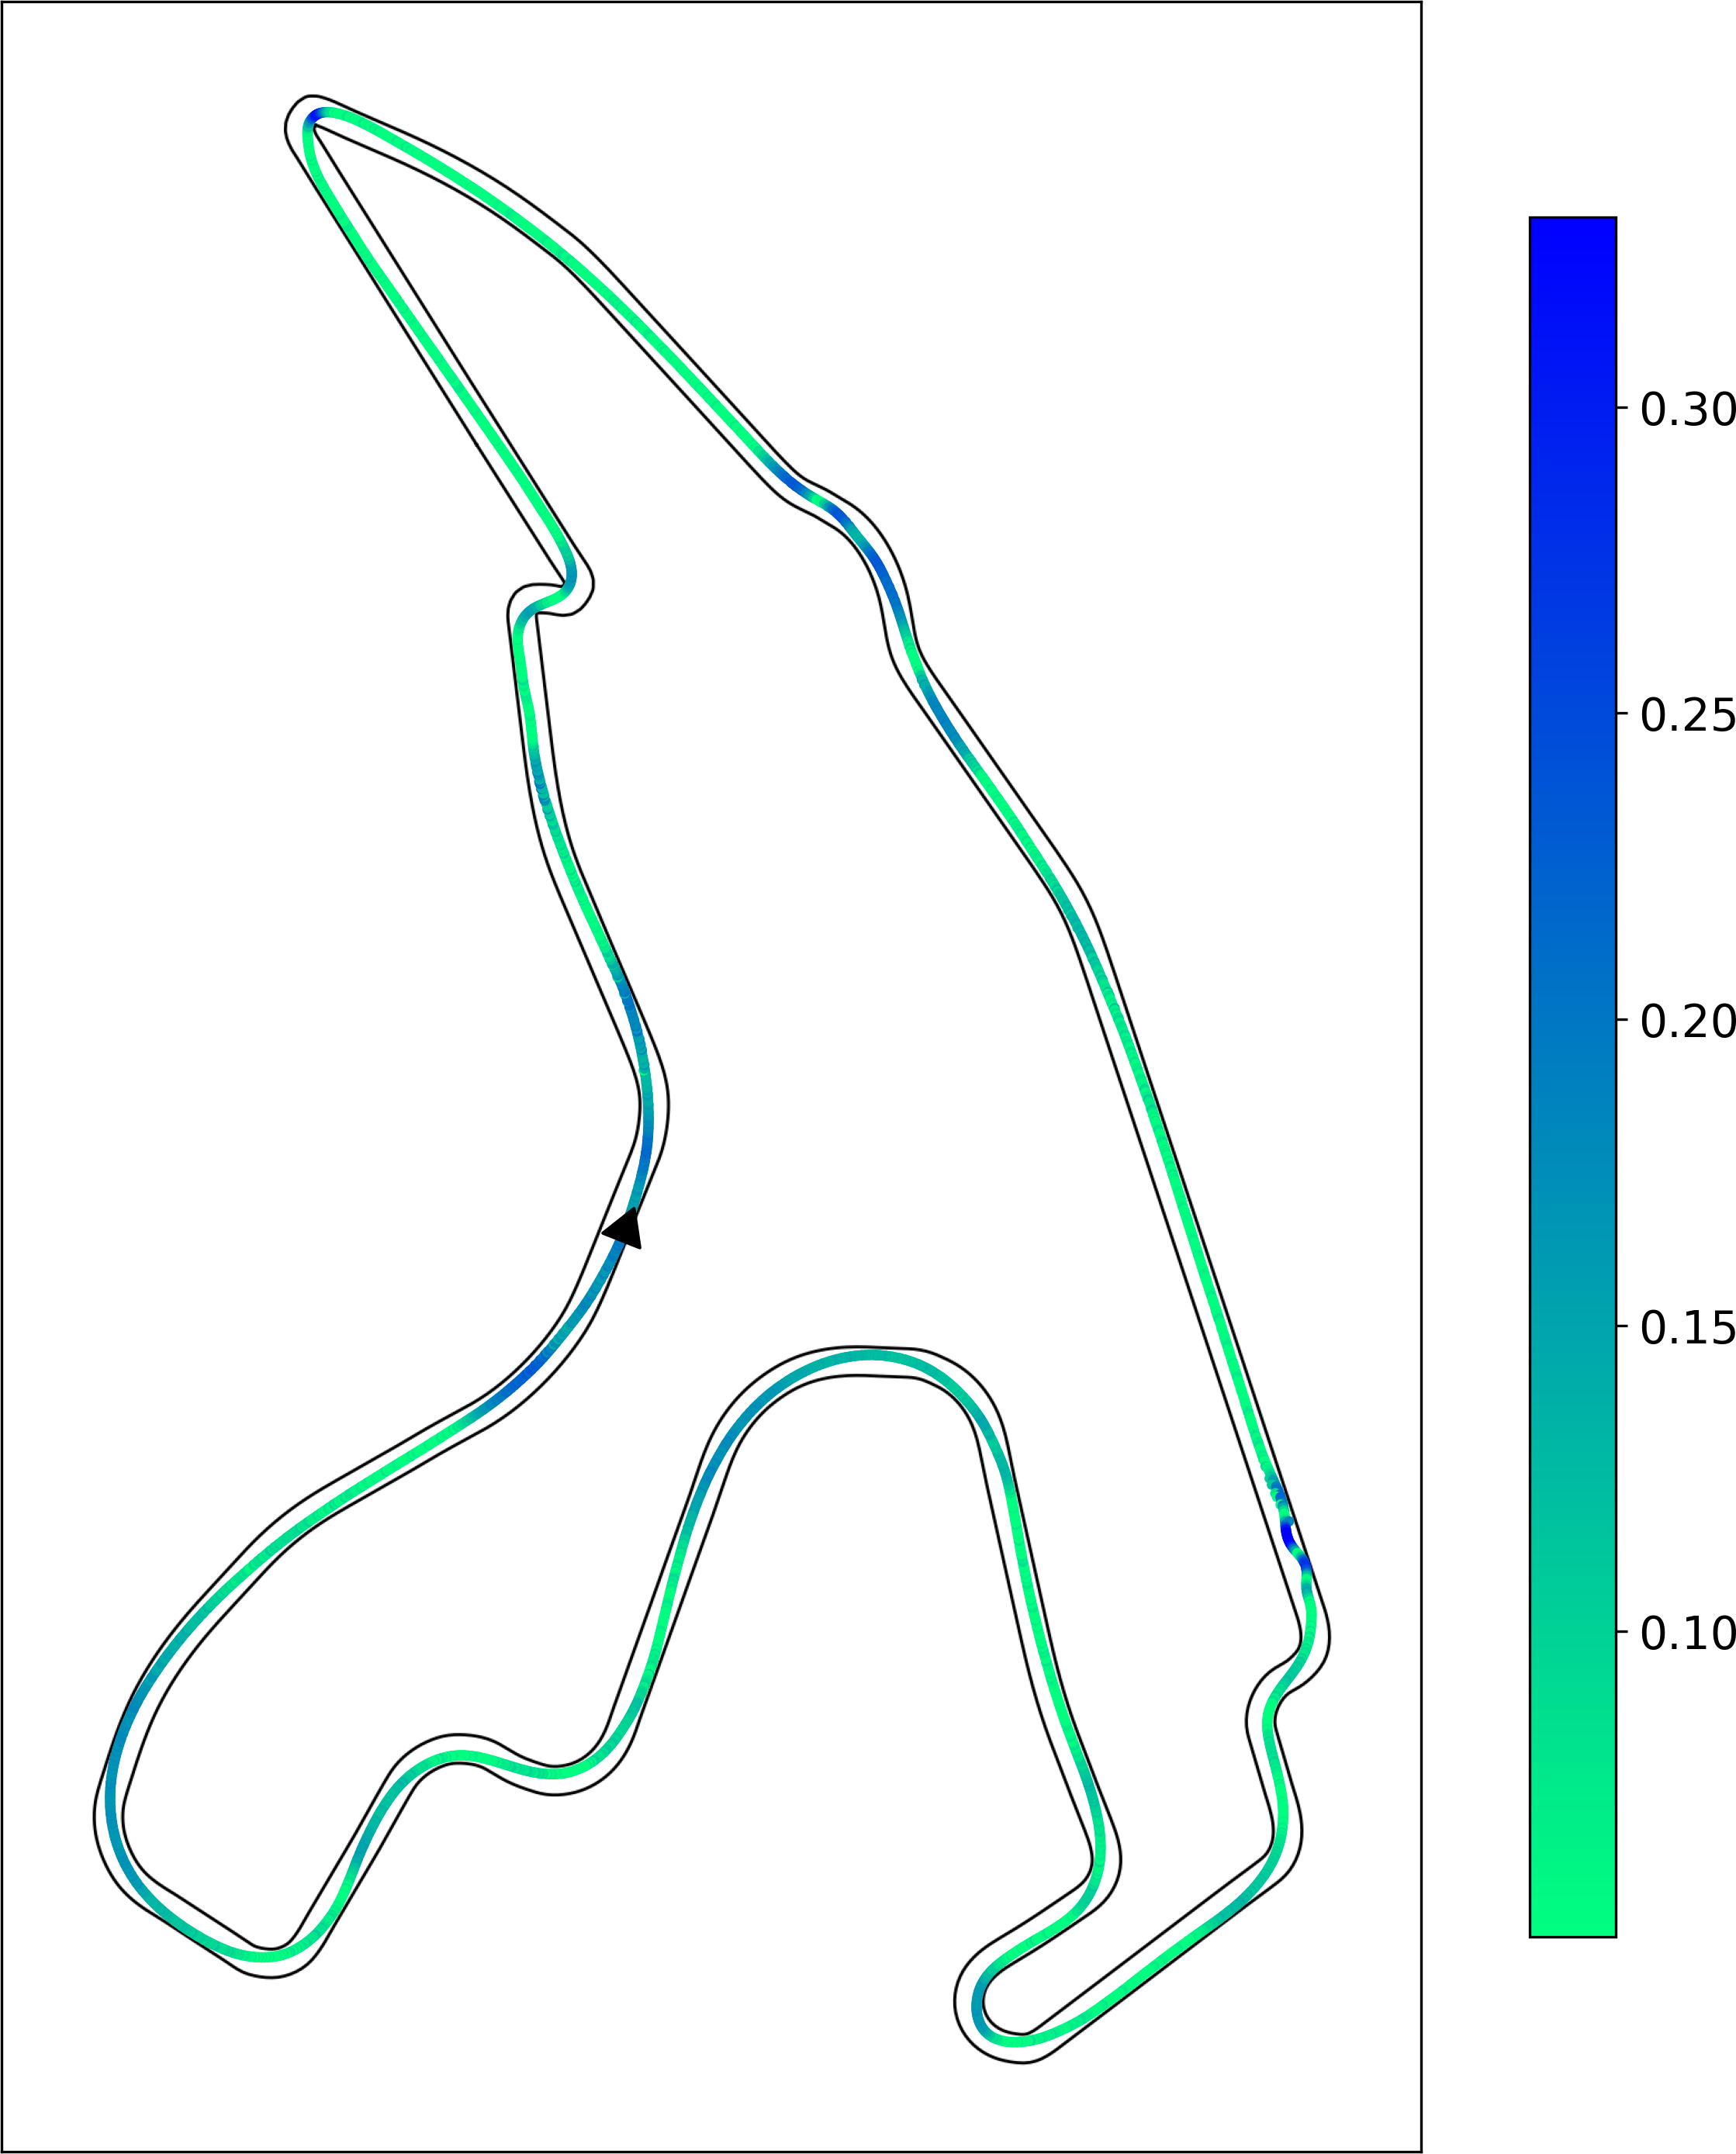
\includegraphics[width=\textwidth]{images/spa_mpc_safe_crosstrack.png}
        \caption{\textit{Safe}}
        \label{fig:tracking_safe_spa}
    \end{subfigure}
    \caption{Crosstrack Error per \textit{Spa}.}
    \label{fig:fig18} % etichetta utilizzata per riferisi all'immagine
\end{figure}
\begin{figure}[H]
    \centering
    \begin{subfigure}[b]{0.3\textwidth}
        \centering
        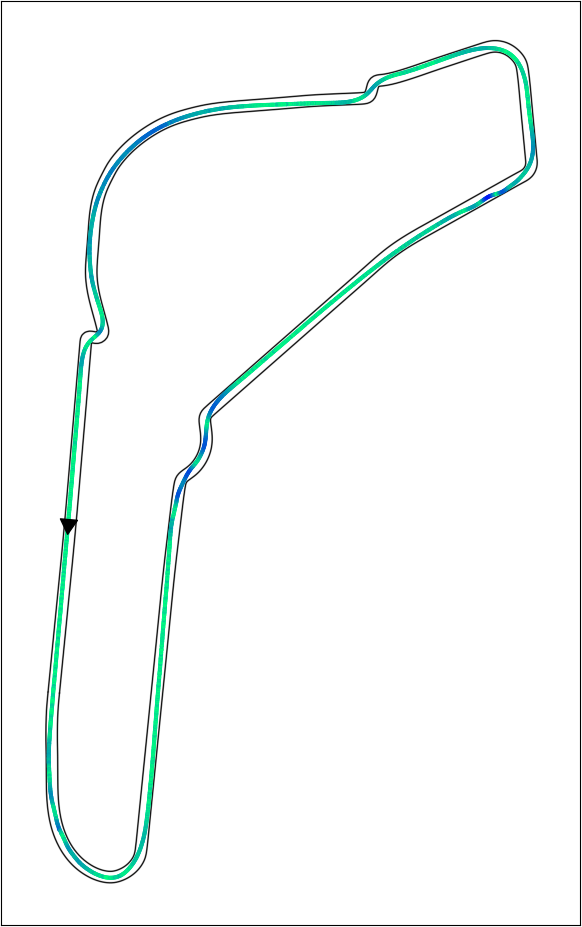
\includegraphics[width=\textwidth]{images/monza_mpc_hp_crosstrack.png} 
        \caption{\textit{High Performance}}
        \label{fig:tracking_hp_monza}
    \end{subfigure}
    \hfill
    \begin{subfigure}[b]{0.3\textwidth}
        \centering
        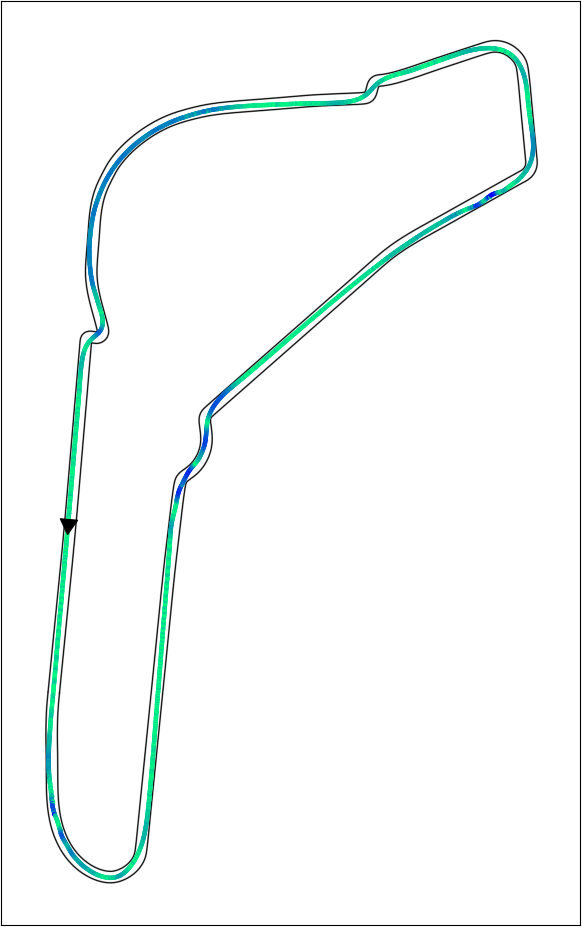
\includegraphics[width=\textwidth]{images/monza_mpc_fast_crosstrack.png}
        \caption{\textit{Fast}}
        \label{fig:tracking_fast_monza}
    \end{subfigure}
    \hfill
    \begin{subfigure}[b]{0.369\textwidth}
        \centering
        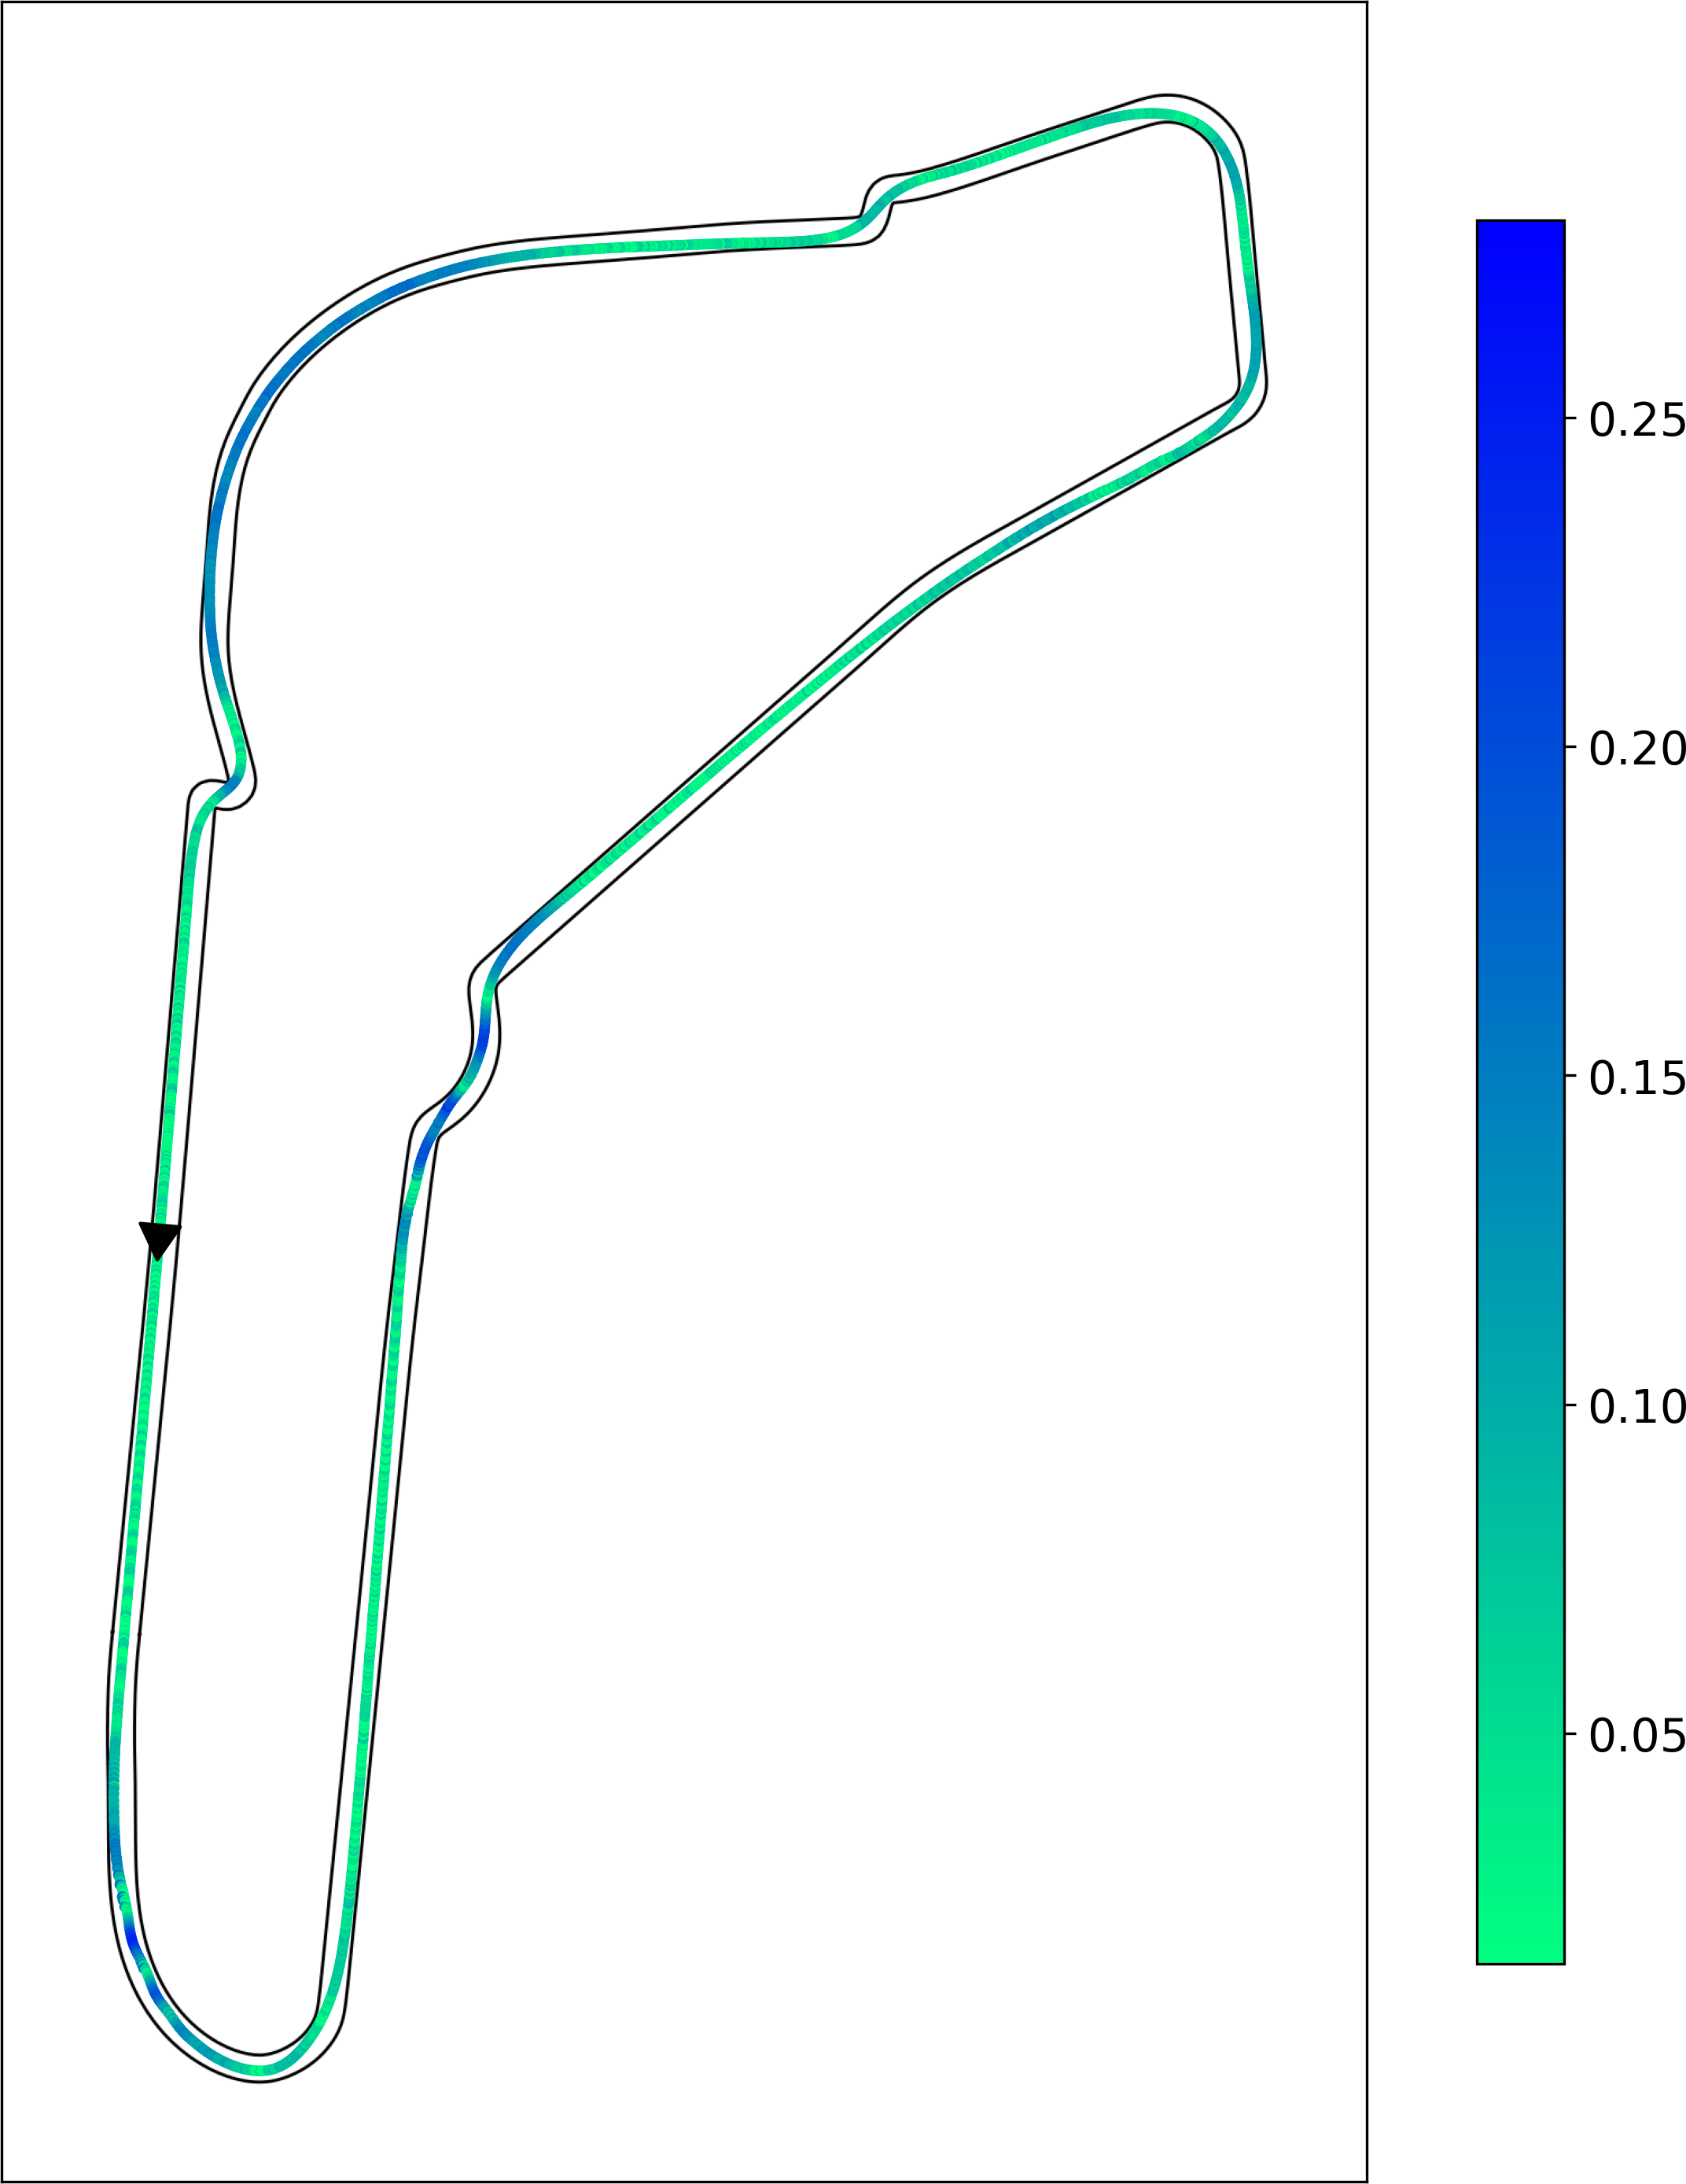
\includegraphics[width=\textwidth]{images/monza_mpc_safe_crosstrack.png}
        \caption{\textit{Safe}}
        \label{fig:tracking_safe_monza}
    \end{subfigure}
    \caption{Crosstrack Error per Monza.}
    \label{fig:fig19} % etichetta utilizzata per riferisi all'immagine
\end{figure}
La situazione è pressoché identica anche per i grafici della pista di 
\textit{Monza}, visualizzati nella Fig.~\ref{fig:fig19}. Unendo i 
risultati riepilogati nella sezione~\ref{subs:metrics}, con questi più 
quelli delle traiettorie mostrate in precedenza, si ottiene un quadro completo
relativo alle discrepanze tra i valori reali e quelli ideali, 
specialmente per quanto riguarda la deviazione dalla linea di riferimento, che è ciò si vuole minimizzare con \textit{MPC}.

\subsection{Velocità e Angolo di sterzata}
Si mostrano di seguito i grafici relativi al confronto della \textit{velocità} e 
dell'\textit{angolo di sterzata} per ogni zona dei due circuiti. Si precisa che viene mostrato
un valore ogni 10 metri per migliorare la resa grafica, così da notare maggiormente le differenze.

\begin{figure}[H]
    \centering
    \begin{subfigure}{\textwidth}
        \centering
        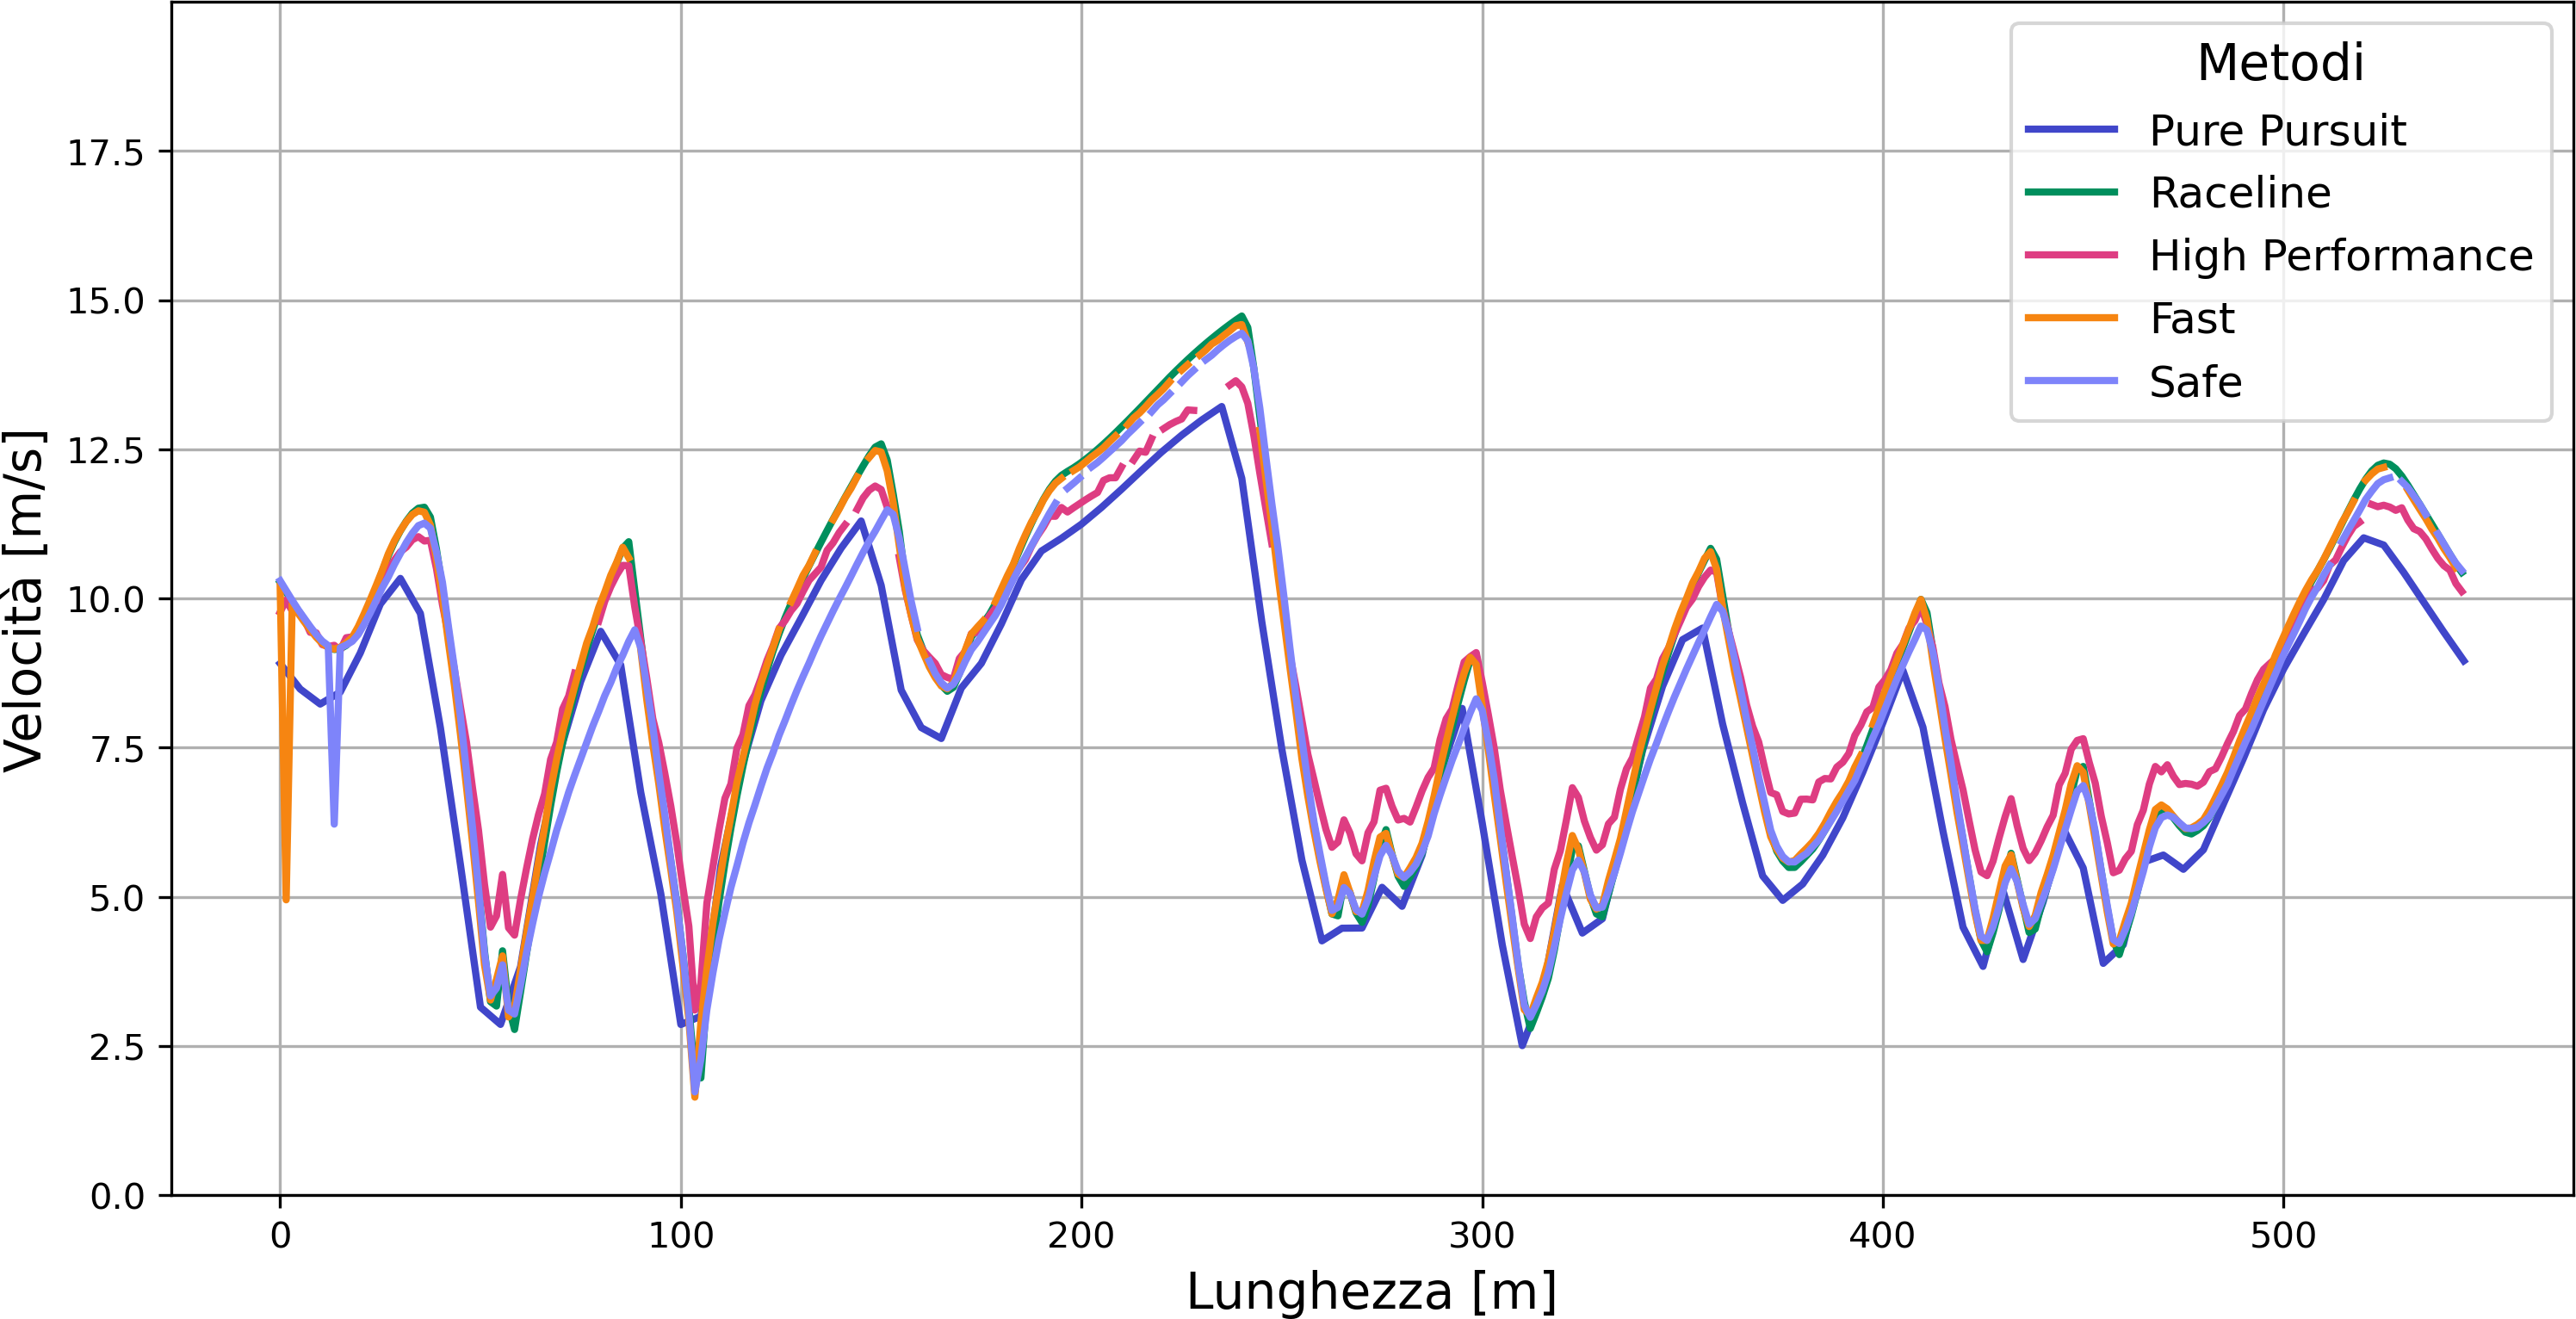
\includegraphics[scale=0.4]{images/spa_mpc_speed_comparisons.png} 
        \caption{\textit{Spa}}
        \label{fig:speed_comp_spa}
    \end{subfigure}
    %\vfill
    \begin{subfigure}{\textwidth}
        \centering
        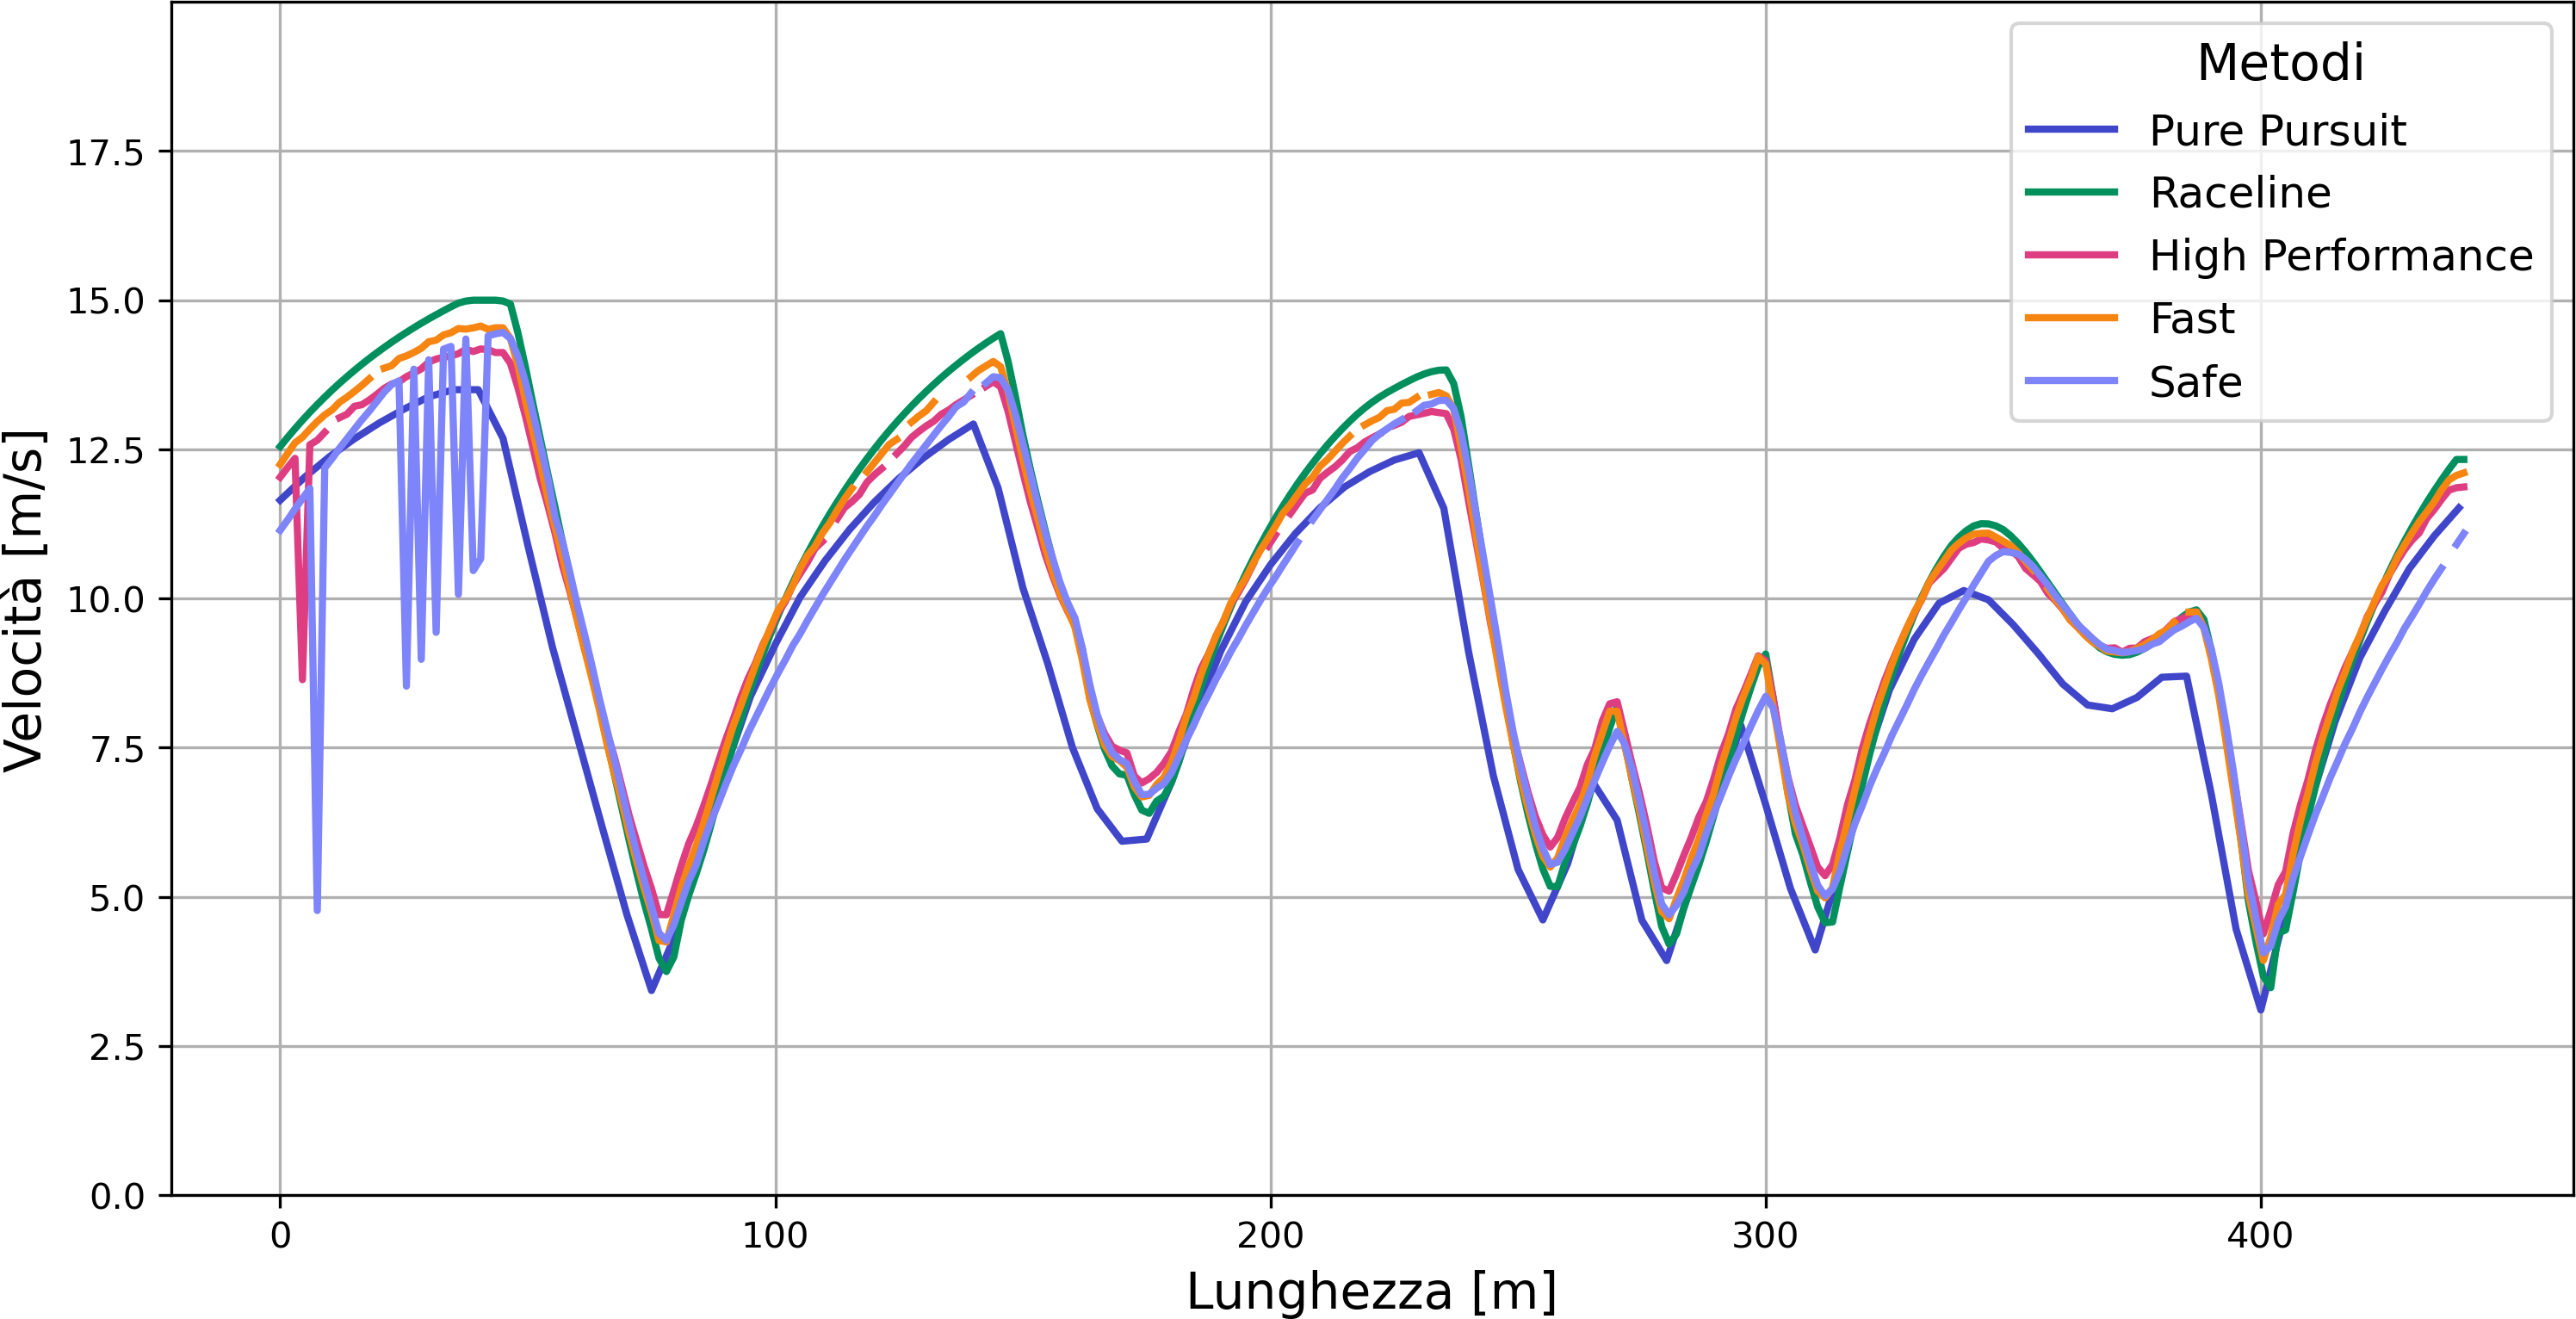
\includegraphics[scale=0.4]{images/monza_mpc_speed_comparisons.png}
        \caption{\textit{Monza}}
        \label{fig:speed_comp_monza}
    \end{subfigure}
    \caption{Confronto delle velocità su \textit{Spa} e \textit{Monza}.}
    \label{fig:fig20} % etichetta utilizzata per riferisi all'immagine
\end{figure}

Per quanto riguarda la velocità, si può osservare in Fig.~\ref{fig:fig20}
come i valori in \textit{Pure Pursuit} restino sempre inferiori agli
altri metodi: ciò accade poiché ha un profilo di velocità corrispondente al
90\% di quello indicato nel dataset della \textit{raceline}. Invece, per tutti
i profili di \textit{MPC}, nei primi 50 metri circa della pista di Monza,
si osserva una notevole variazione nella velocità applicata dall'algoritmo. 
Ciò è dovuto a un iniziale tempo di assestamento, in particolare per il profilo
\textit{Safe MPC} dato che parte più lentamente rispetto agli altri e con
un'accelerazione di 10 m/s$^2$.
Al contrario, gli altri profili mostrano un comportamento più attenuato, poiché
iniziano con velocità più elevate e un'accelerazione di 3 m/s$^2$.
Invece, si può osservare nella Fig.~\ref{fig:fig21} quanto appena descritto da un punto
di vista qualitativo, dove è stata riportata solo la parte iniziale del giro di 
\textit{Monza}. Si precisa che la scala cromatica è basata sui valori di velocità
della \textit{raceline} ottimale. In più, si osservino le variazioni cromatiche dei punti nello \textit{scatter plot}.

\begin{figure}[H]
    \centering
    \begin{subfigure}[b]{0.3\textwidth}
        \centering
        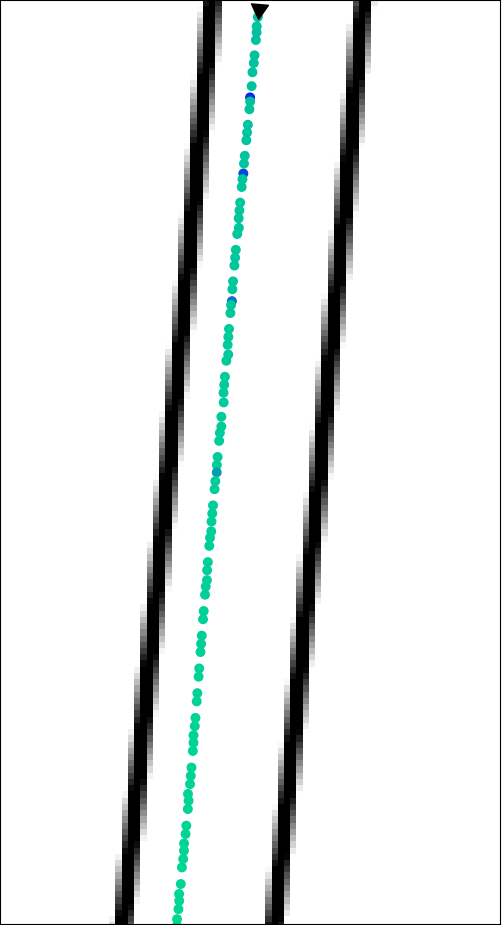
\includegraphics[width=\textwidth]{images/monza_zoom_mpc_high_performance_speed.png} 
        \caption{\textit{High Performance}}
        \label{fig:hp_speed}
    \end{subfigure}
    %\hfill
    \begin{subfigure}[b]{0.29\textwidth}
        \centering
        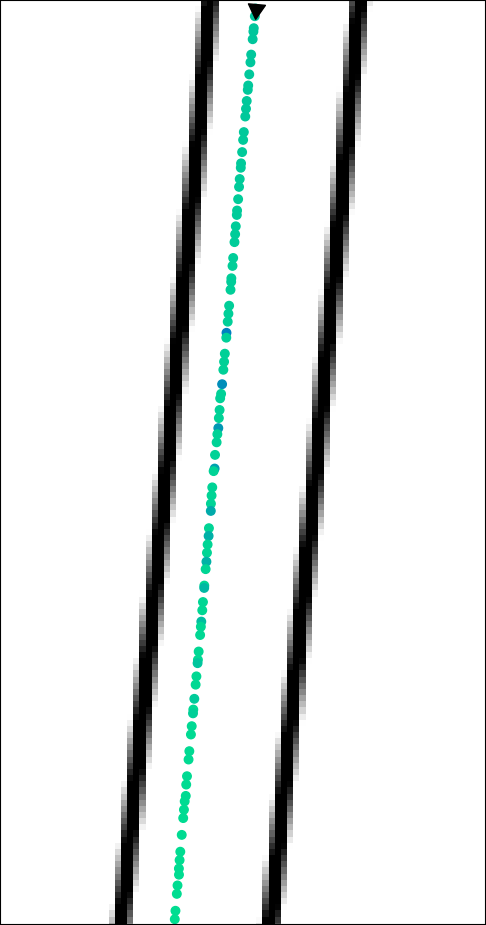
\includegraphics[width=\textwidth]{images/monza_zoom_mpc_fast_speed.png}
        \caption{\textit{Fast}}
        \label{fig:fast_speed}
    \end{subfigure}
    %\hfill
    \begin{subfigure}[b]{0.3805\textwidth}
        \centering
        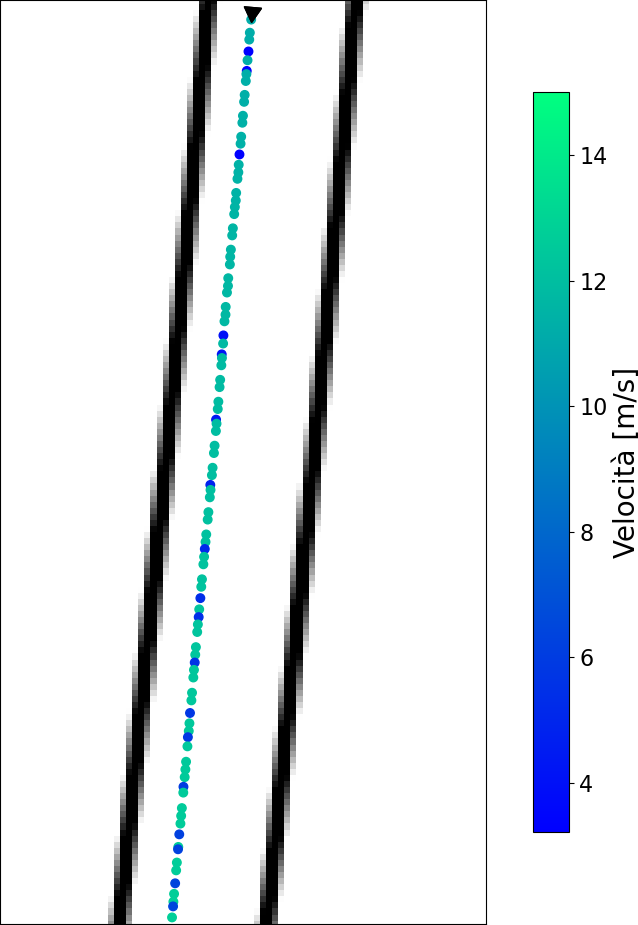
\includegraphics[width=\textwidth]{images/monza_zoom_mpc_safe_speed.png}
        \caption{\textit{Safe}}
        \label{fig:safe_speed}
    \end{subfigure}
    \caption{Confronto tra i metodi di \textit{MPC} su \textit{Monza}.}
    \label{fig:fig21} % etichetta utilizzata per riferisi all'immagine
\end{figure}

Dopo questa fase iniziale, per la pista di \textit{Monza} le velocità 
dei tre metodi sono molto simili a quella di riferimento data dalla 
\textit{raceline ottima}. Invece, per quella di \textit{Spa}, il profilo
\textit{High Performance} tende a superare la velocità di riferimento dalla seconda metà del tracciato.

Viene visualizzato graficamente anche l'angolo di sterzata $\delta$ attraverso il confronto dei
valori applicati dal \textit{Pure Pursuit} con quelli delle tre configurazioni di \textit{MPC}.

\begin{figure}[H]
    \centering
    \begin{subfigure}{\textwidth}
        \centering
        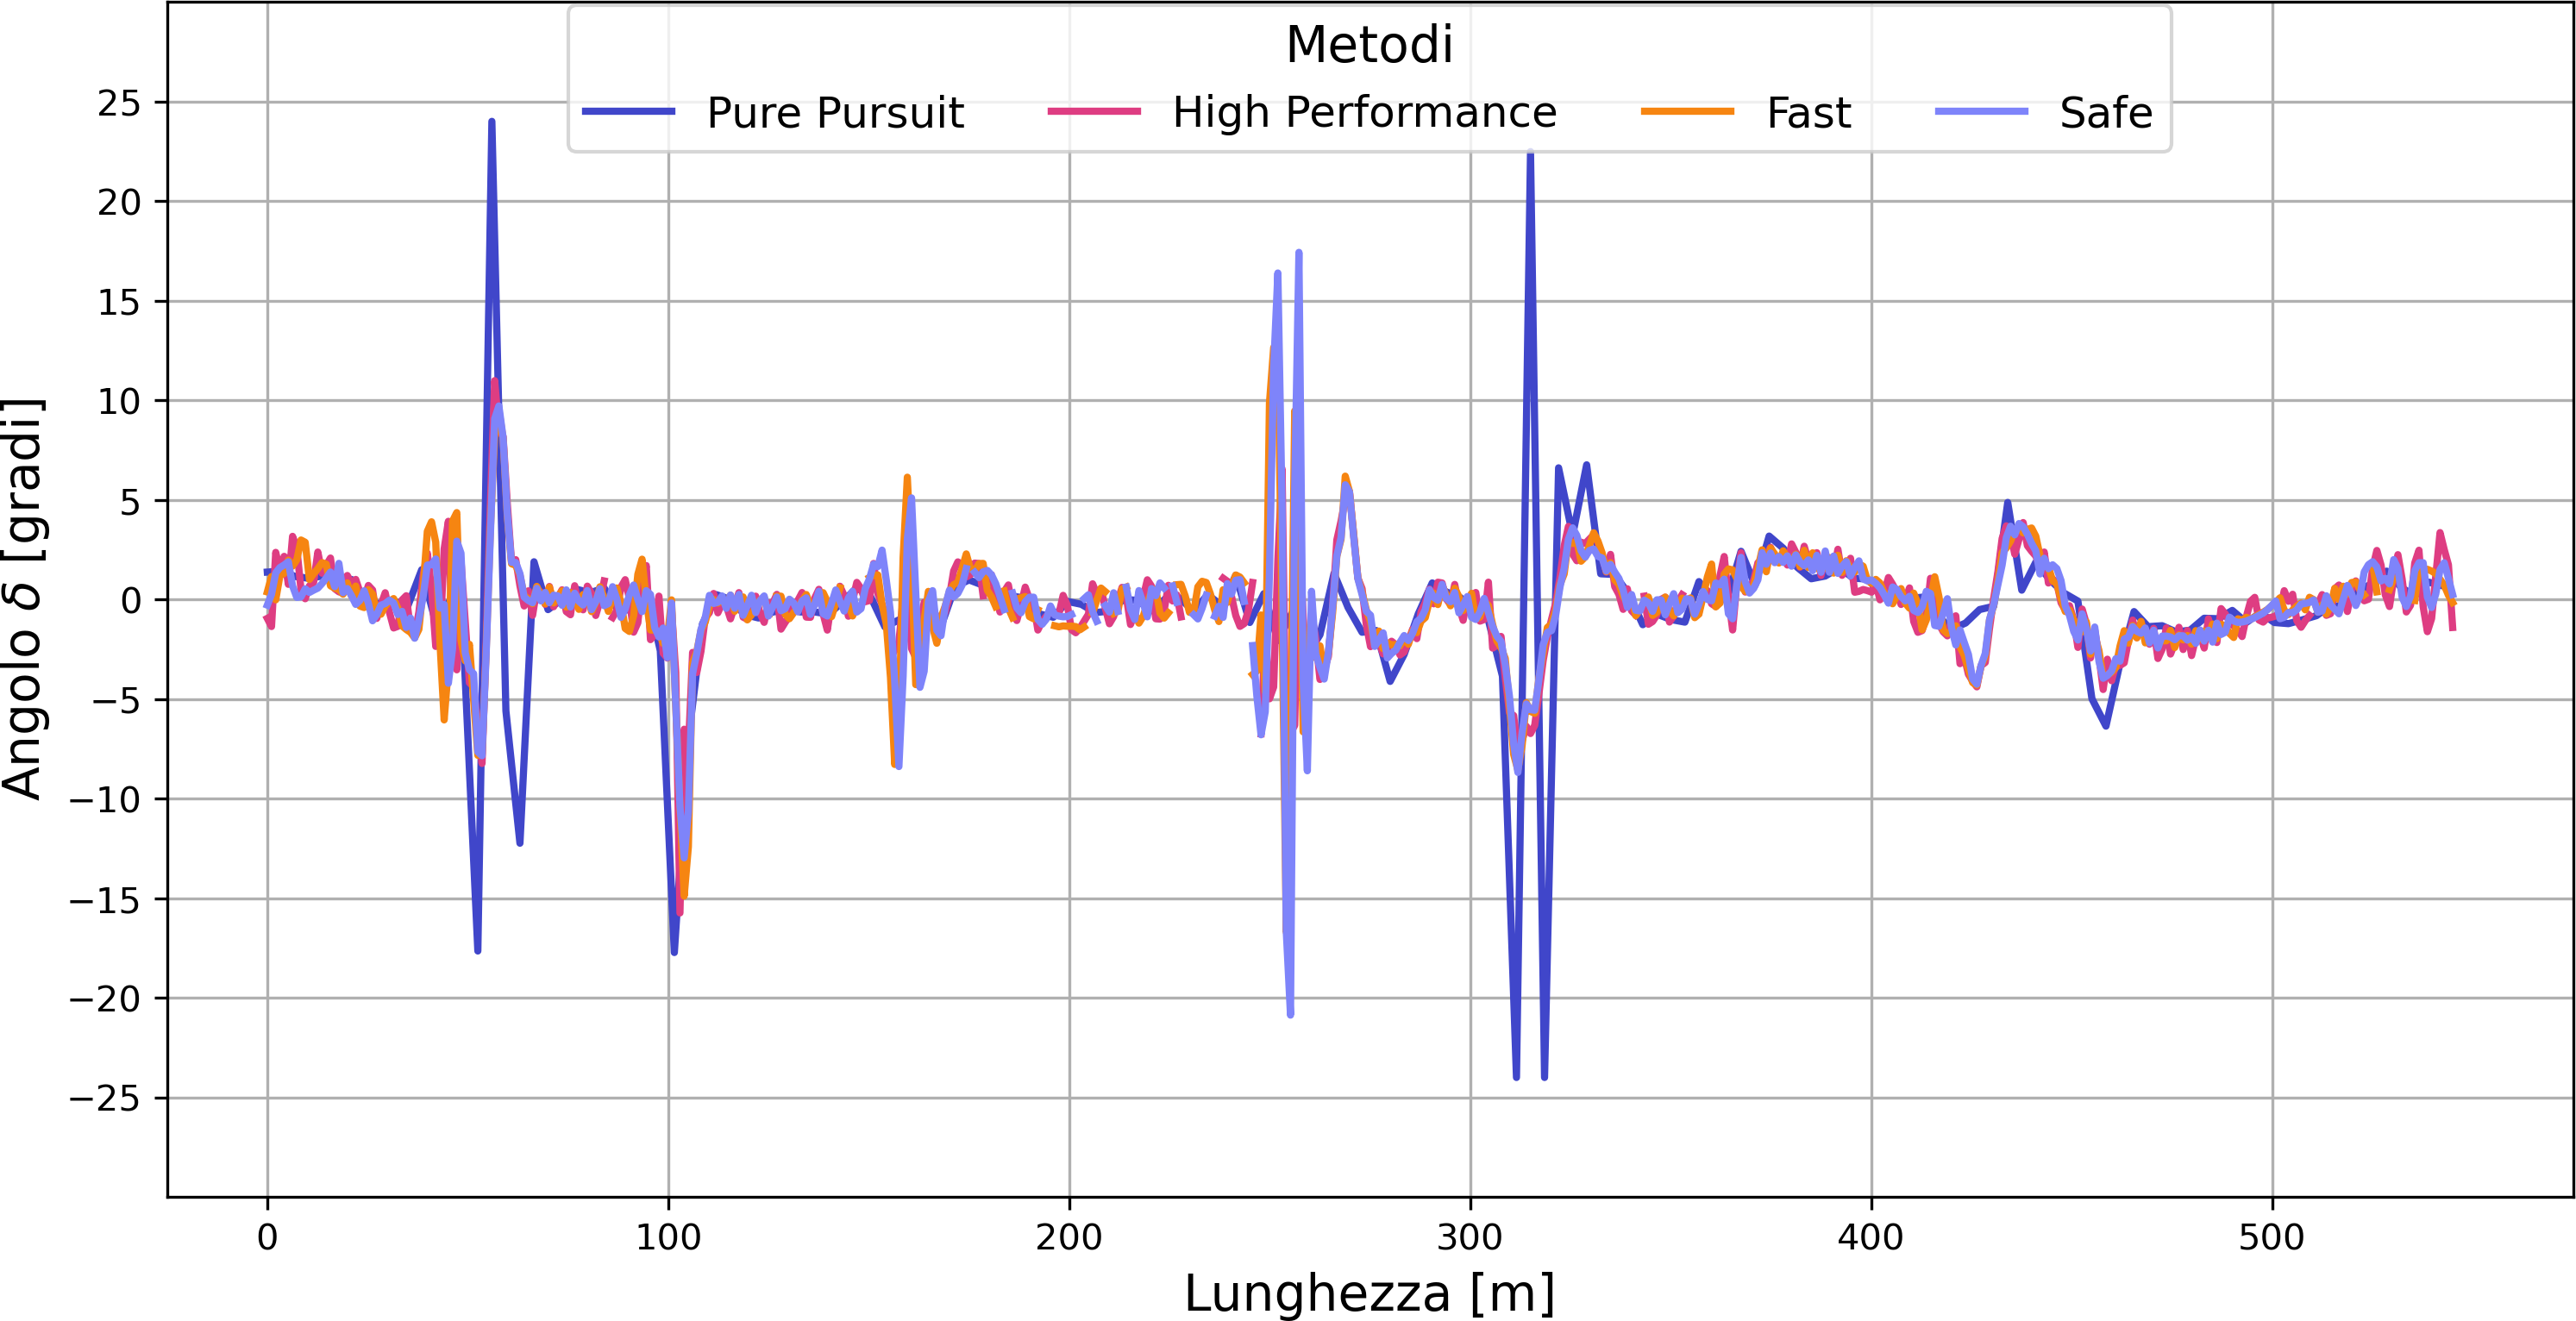
\includegraphics[scale=0.4]{images/spa_mpc_theta_comparisons.png} 
        \caption{\textit{Spa}}
        \label{fig:delta_comp_spa}
    \end{subfigure}
    %\vfill
    \begin{subfigure}{\textwidth}
        \centering
        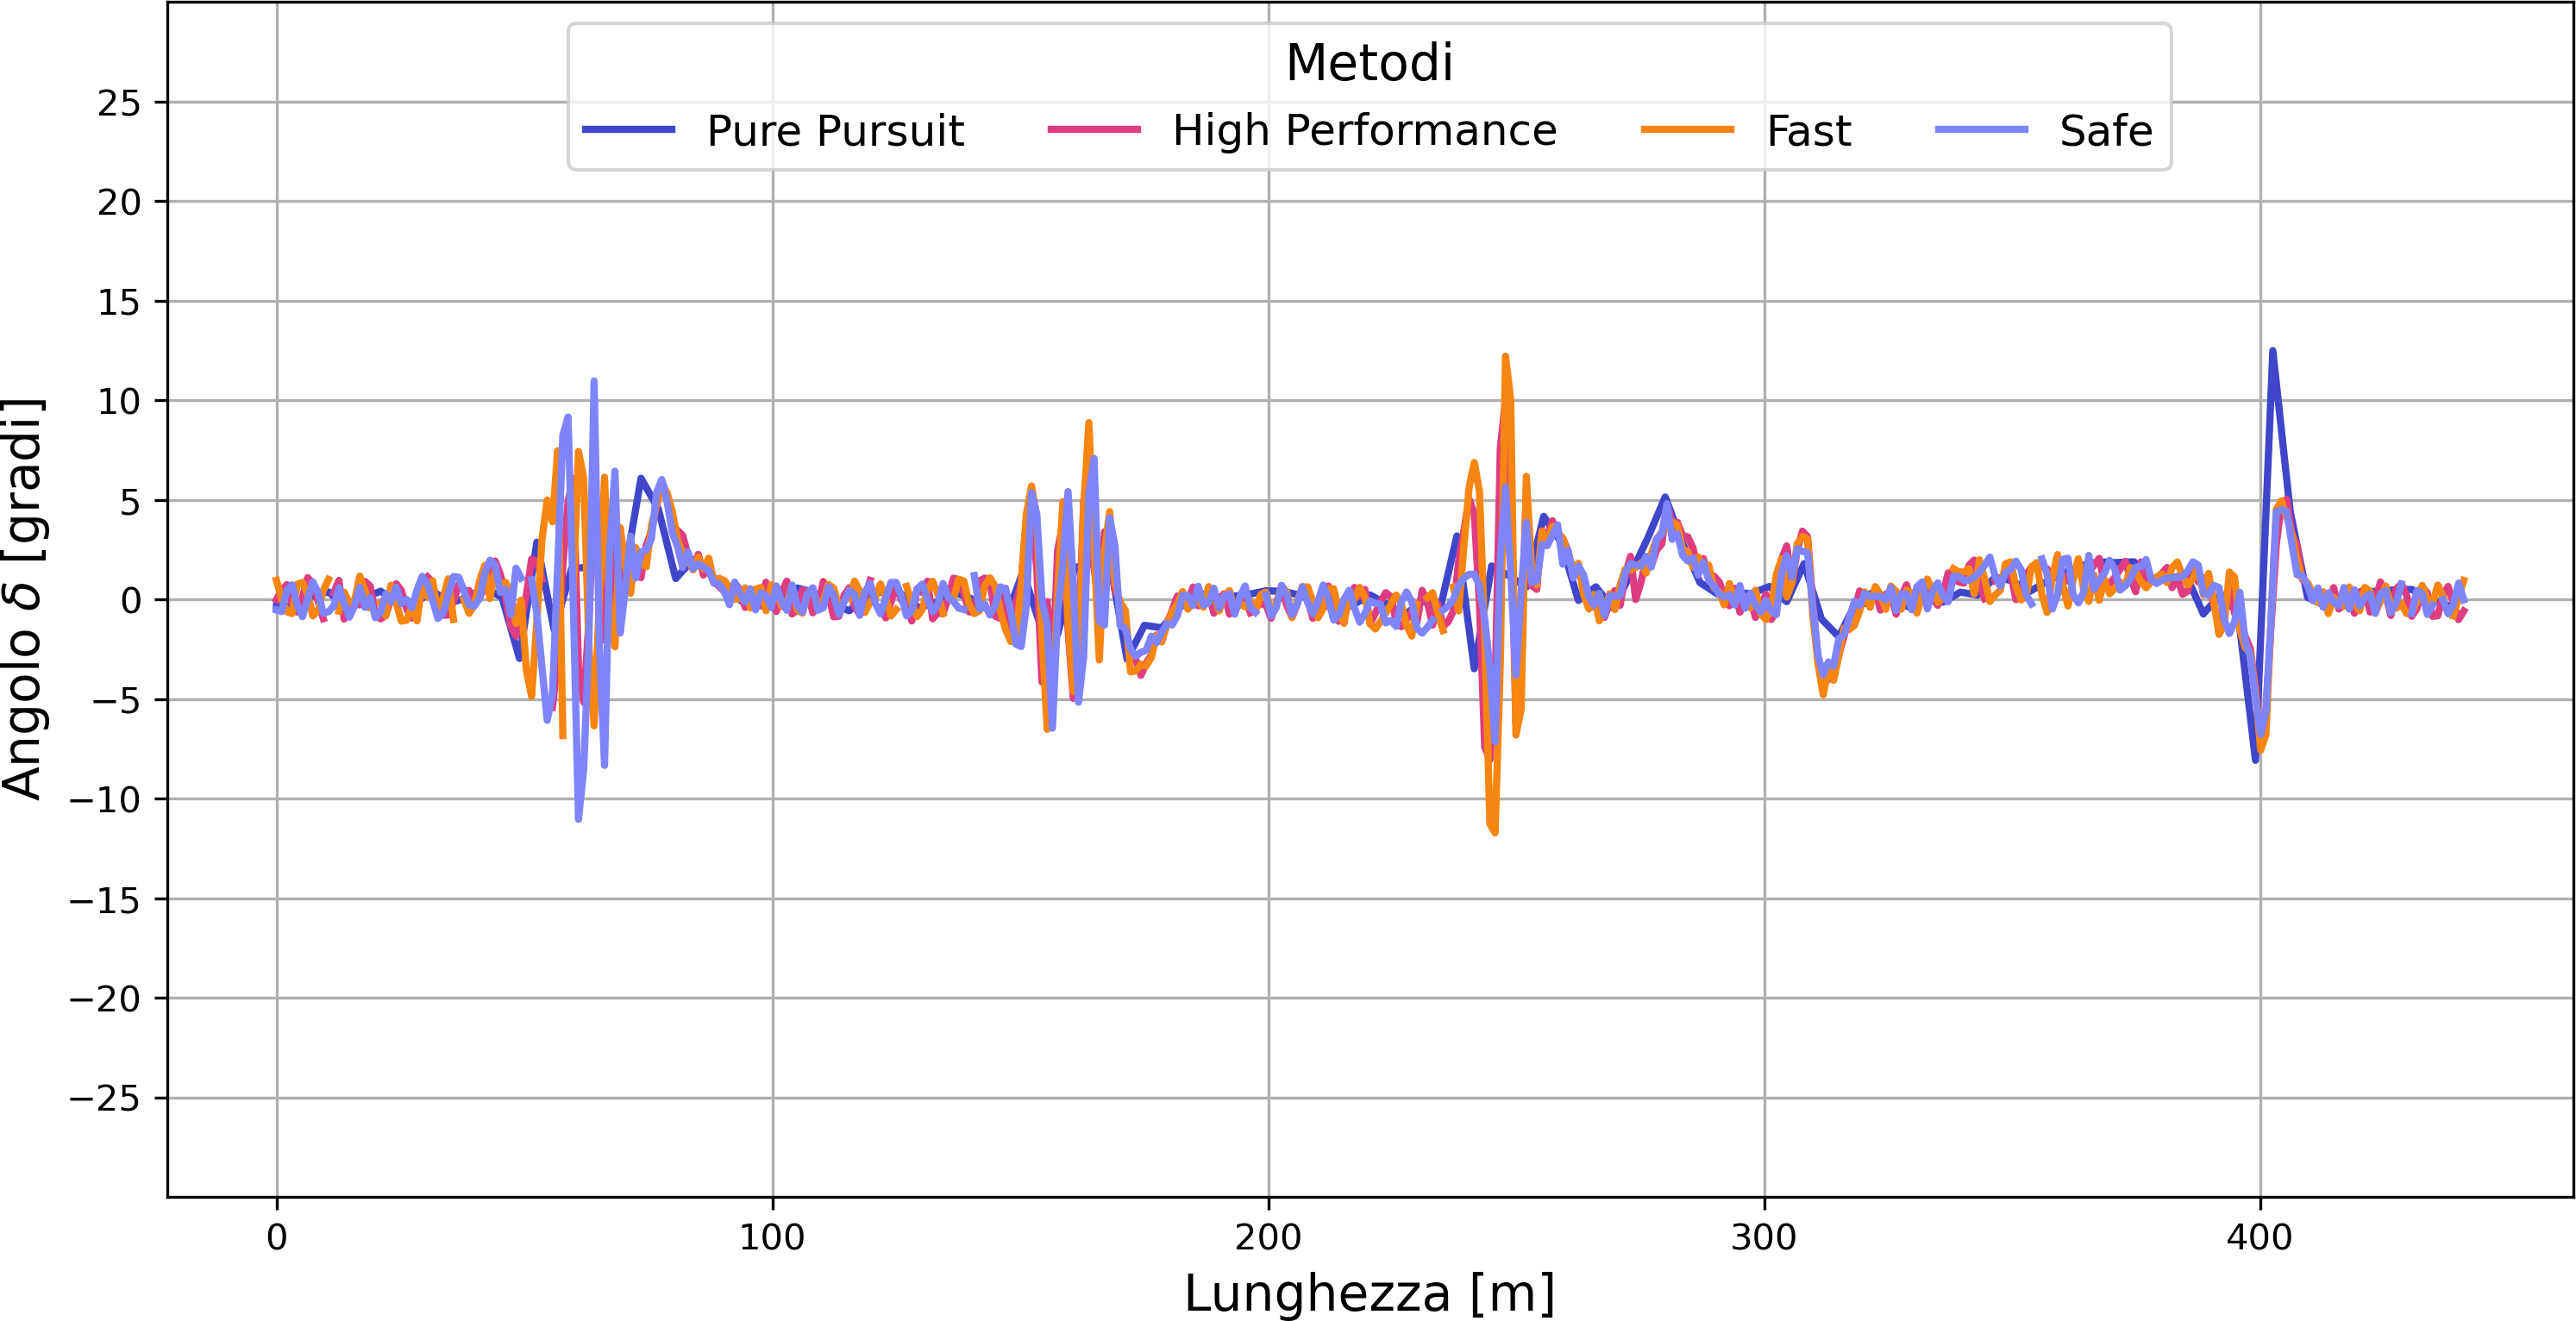
\includegraphics[scale=0.4]{images/monza_mpc_theta_comparisons.png}
        \caption{\textit{Monza}}
        \label{fig:delta_comp_monza}
    \end{subfigure}
    \caption{Confronto degli angoli di sterzata applicati su \textit{Spa} e \textit{Monza}.}
    \label{fig:fig22} % etichetta utilizzata per riferisi all'immagine
\end{figure}
Come mostrato in Fig.~\ref{fig:fig22}, il \textit{Pure Pursuit} presenta 
angoli di sterzata massimi più elevati in specifici punti di \textit{Spa} 
rispetto a Monza, mentre altrove è generalmente simile a \textit{MPC}.
Infatti, i profili \textit{MPC} mostrano angoli analoghi tra loro
su \textit{Spa}, con aumenti in certe zone per \textit{Safe} e 
\textit{Fast}, ma anche su \textit{Monza} si ha un comportamento simile. 
Dunque, in generale, i profili di \textit{MPC} hanno applicato angoli
assimilabili a quelli di \textit{Pure Pursuit}, a eccezione di certe zone di \textit{Spa}.